\documentclass[conference,compsoc]{IEEEtran}
% *** CITATION PACKAGES ***
%
\ifCLASSOPTIONcompsoc
  % IEEE Computer Society needs nocompress option
  % requires cite.sty v4.0 or later (November 2003)
  \usepackage[nocompress]{cite}
\else
  % normal IEEE
  \usepackage{cite}
\fi
\usepackage[export]{adjustbox}

\usepackage{microtype}
\usepackage{booktabs} % for professional tables





\usepackage{graphicx} % "demo" option just for this example
\usepackage{subcaption}

\usepackage{amsmath}
\usepackage{booktabs,subcaption,amsfonts,dcolumn}



\usepackage{graphicx} % "demo" option just for this example
\usepackage{subcaption}

\usepackage{booktabs,subcaption,amsfonts,dcolumn}
\newcolumntype{d}[1]{D..{#1}}
\newcommand\mc[1]{\multicolumn{1}{c}{#1}} % handy shortcut macro


\usepackage{booktabs,subcaption,amsfonts,dcolumn}
\newcolumntype{d}[1]{D..{#1}}


\usepackage[usenames, dvipsnames]{color}
\newcommand{\ts}{\textsuperscript}

\usepackage{graphicx}

\graphicspath{{/home/danai/Documents/SVM_latex/figures/}{/home/danai/Music/Documents/SVM_latex/figures}}
% *** GRAPHICS RELATED PACKAGES ***
%
\ifCLASSINFOpdf

\hyphenation{op-tical net-works semi-conduc-tor}

\usepackage{tabularx} % in the preamble
\begin{document}
%
\title{\line(1,0){250}\\Support Vector Machines Methods and Applications\\\line(1,0){250}}
%\title{[H02C4A] Artificial Neural Networks and Deep Learning}


\author{\IEEEauthorblockN{Danai Triantafyllidou}
\\
	\IEEEauthorblockA{Master of Artificial Intelligence, KU Leuven\\
	\\2018-2019
	\vspace{1cm}
	}
}


\onecolumn

%\listoffigures
% 
%\listoftables
\maketitle




%\newpage
%\tableofcontents
%\listoffigures
%\listoftables
\IEEEpeerreviewmaketitle




\thispagestyle{plain}
\pagestyle{plain}
\onecolumn

%\tableofcontents
\section{Exercise Session 1}
\subsection{A simple example: two Gaussians}

For a binary classification problem, the Bayes classification rule leads to a minimal probability of misclassification. According to Bayes rule, a test observation $x$ is assigned to a class $i^*$ so that $i^* = arg \max\limits_{i,\dots 2} P(C_i|x)$, where $P(C_i|x)$ denotes the posterior class probability of class $C_i$. This also corresponds to minimizing the overlap area between the distributions $P(C_1|x)P(C_1)$ and $P(C_2|x)P(C_2)$. If the data are generated from a Gaussian distribution with the same covariance matrix for the two classes, the optimal decision boundary is a linear seperating hyperplane which is independent of the overlap area between these Gaussian distributions. As a consequence, in the case of non-seperable classes with overlapping distributions, misclassifications should be tolerated.


\subsection{Support vector machine classifier}

Consider a given training set $\{x_k,y_k\}^N_{k=1}$ with input data $x_k \in \mathcal{R}^N $ and output data $y_k \in \mathcal{R} $ with class labels $y_k \in \{-1,+1 \}$. According to Vapnik's extension of linear Support Vector Machines (SVMs) to the non-seperable case, the optimization problem in its primal form becomes:

\begin{equation}
\min\limits_{w,b,\xi} J(w,b) = \frac{1}{2}w^Tw + c \sum_{k=1}^{N}\xi_k
\end{equation}
subject to
\begin{equation*}
\begin{cases}
\begin{aligned}
  y_k[w^Tx_k+b] \geq 1-\xi_k, k=1,...,N \\
  \xi_k \geq 0, k =1,...N
\end{aligned}
\end{cases}
\end{equation*}
where $\xi_k$ slack variables measure the distance of each data point $x_k$ from the marginal hyperplane. Slack variables allow a data point $x_k$ example to be in the margin ($0< \xi<1$), or to be misclassified ($\xi>1$).
The term $c \sum_{k=1}^{N}\xi_k$ is used to penalize misclassification and margin errors. Additions on the wrong side of the hyperplane drastically change the decision boundary as they increase the value of the penalization term, as opposed to additions on the correct side of the hyperplane that have a minor impact to the solution. This behavior is illustrated in Figure~\ref{fig:adding}. 



   \begin{figure*}[]
        \begin{subfigure}{0.33\linewidth}
            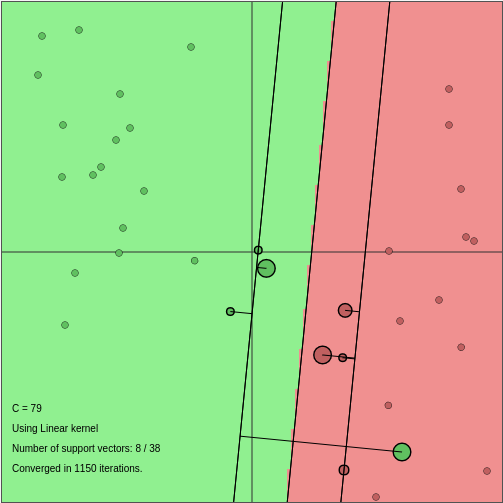
\includegraphics[width=\linewidth]{add1}
            \caption{original solution}
        \end{subfigure}
        \begin{subfigure}{0.33\linewidth}
            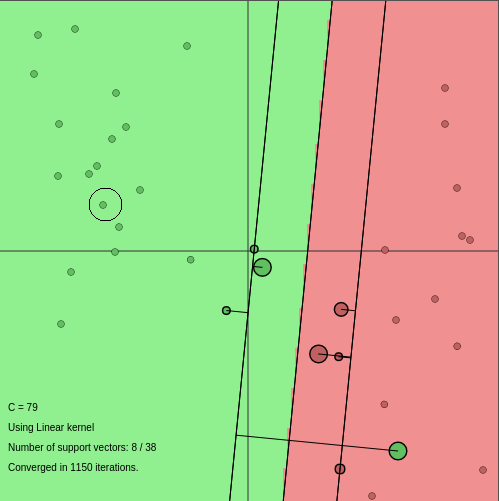
\includegraphics[width=\linewidth]{add2}
            \caption{new green data point on the right side}
        \end{subfigure}
        \begin{subfigure}{0.33\linewidth}
            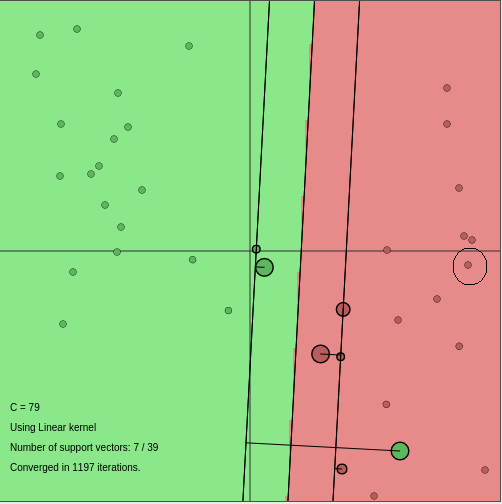
\includegraphics[width=\linewidth]{add3}
            \caption{new red data point on the right side}
        \end{subfigure}


		\begin{subfigure}{0.33\linewidth}
            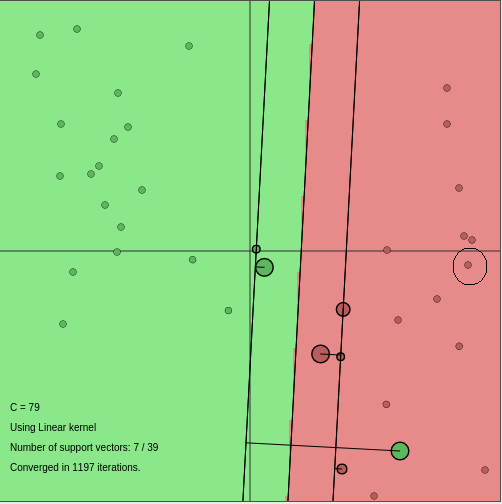
\includegraphics[width=\linewidth]{add3}
            \caption{original solution}
        \end{subfigure}
        \begin{subfigure}{0.33\linewidth}
            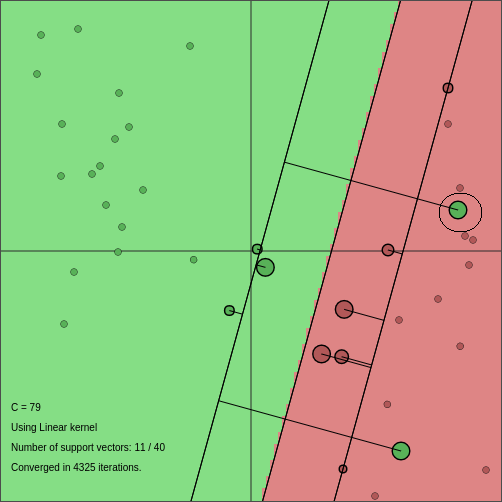
\includegraphics[width=\linewidth]{add4}
            \caption{new green data point on the wrong side}
        \end{subfigure}
        \begin{subfigure}{0.33\linewidth}
            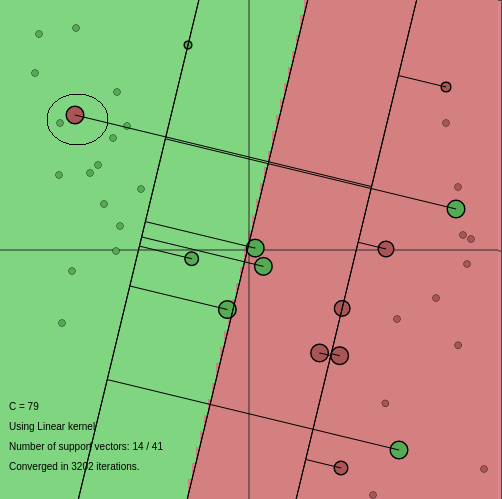
\includegraphics[width=\linewidth]{add5}
            \caption{new red data point on the wrong side}
        \end{subfigure}
   
 	
        \caption{Visualizing the change in the hyperplane by adding more data points}
        
        
       
    
        
        \label{fig:adding}
    \end{figure*}


The regularization hyperparameter c determines how much emphasis is put on maximizing the margin versus tolerating misclassification errors. For a large value of c, a large penality is assigned to misclassification/margin errors. A smaller value for c, allows to ignore points close to the boundary, and increases the margin. Putting more emphasis on minimizing the norm $||w||$ instead of minimizing the errors $\sum_{k=1}^{N}\xi_k$, also means that the model becomes more flexible. The flexibility of the model is also associated with the classic bias-variance tradeoff. A more flexible model has a smaller bias but a higher variance and is more prone to overfitting. Consequently, using a smaller alue for $c$ creates a model of higher variance that conceptually corresponds to a wider margin. As c is increased, the hyperplane's orientation is changed, and the margin becomes more narrow. Intuitively, by emphasizing the importance of minimizing the classification errors (which means that we use a large $c$) the solution becomes less sparse and the final decision regarding the class involves the contribution of more points. When examining the problem in its dual form, this corresponds to a larger number of non zero $a_k$ variables that contribute to the final solution. For the case of a linear kernel, this effect is illustrated in Figure~\ref{fig:c}. Indeed, higher values of $c$ produce a smaller margin and fewer support vectors. 

\begin{figure*}
        \begin{subfigure}{0.33\linewidth}
            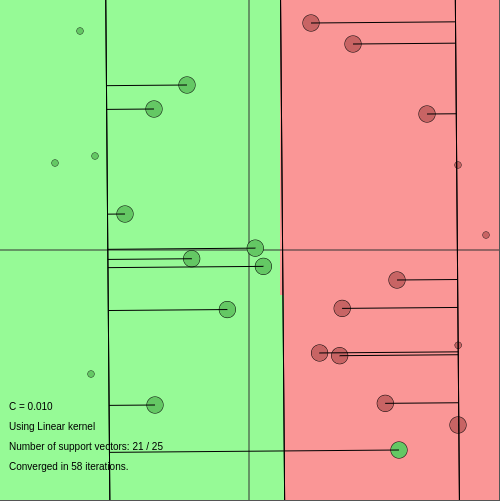
\includegraphics[width=\linewidth]{svmc01}
            \caption{c=0.1}
        \end{subfigure}
        \begin{subfigure}{0.33\linewidth}
            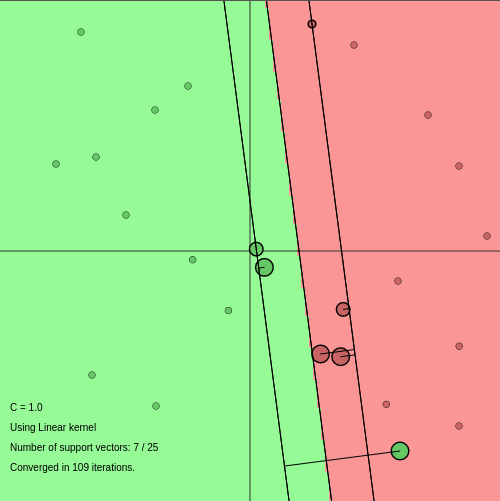
\includegraphics[width=\linewidth]{svmc10}
            \caption{c=1.0}
        \end{subfigure}
        \begin{subfigure}{0.33\linewidth}
            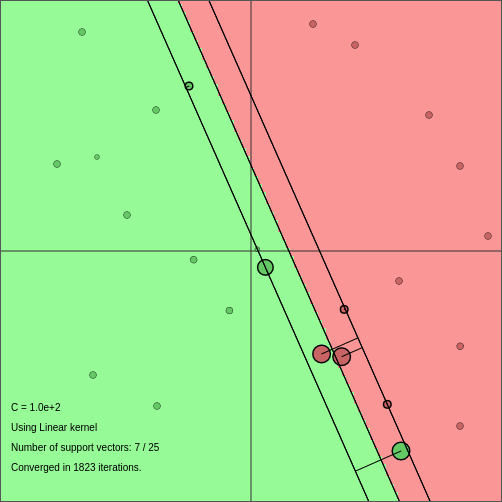
\includegraphics[width=\linewidth]{svmc100}
            \caption{c=100}
        \end{subfigure}

        \caption{Varying the $c$ parameter for the linear kernel }        
                    
        \label{fig:c}
    \end{figure*}
 

Kernel methods have been widely applied to support vector machines, as they allow to operate in a different feature space and construct non linear models. The optimization problem now becomes:

\begin{equation}
\min\limits_{w,b,\xi} J(w,b) = \frac{1}{2}w^Tw + c \sum_{k=1}^{N}\xi_k
\end{equation}
subject to
\begin{equation*}
\begin{cases}
\begin{aligned}
  y_k[w^T\phi(x_k)+b] \geq 1-\xi_k, k=1,...,N \\
  \xi_k \geq 0, k =1,...N
\end{aligned}
\end{cases}
\end{equation*}
where $\phi(x_k)$ can be infinite dimensional. By constructing the lagragian, one can solve the problem in its dual form:


\begin{equation}
\max\limits_{\alpha} J(w,b) = -\frac{1}{2}\sum_{k,l=1}^{N}y_ky_lK(x_k,x_l)\alpha_k\alpha_l +  \sum_{k=1}^{N}\alpha_k
\end{equation}
such that
\begin{equation*}
\begin{cases}
\begin{aligned}
   \sum_{k=1}^{N}\alpha_ky_k=0 \\
  0 \geq a_k \geq c, k =1,...N
\end{aligned}
\end{cases}
\end{equation*}
where $K(x_k,x_l)=\phi(x_k)^T\phi(x_l)$ is the kernel function. The idea behind kernel methods is that if the data is not separable in the original space they can become separable in a higher dimensional space. This is better illustrated in Figure~\ref{fig:example}, for the case of 1-dimensional data. In the left plot, the original data points are shown which are not linearly separable in this 1-dimensional space. After applying the transformation $\phi(x)=x^2$ a second dimension is added to the feature space and the classes become linearly separable.

The kernel trick allows to work in feature spaces without actually needing to perform any computations in this space. The power of kernel methods lies exactly in their ability to represent the data only through a set of pairwise similarity comparisons between the original data observations (by using their original coordinates in the lower dimensional space), instead of explicitly applying the transformation $\phi()$. Finally, in order to predict the class of a new test instance $x$ with a SVM classifier, a linear combination of kernel evaluations between the test instance and all the non-zero lagragian $\alpha$ variables should be computed:
  

\begin{equation}
y(x) = sign[\sum_{k=1}^{N}\alpha_ky_kK(x,x_k) +b ]
\end{equation}
A property of the SVM is that the solution vector is sparse, which means that many of the resulting $a_k$ values of equation (4) will be zero. The  sum $\sum_{k=1}^{\#SV}\alpha_ky_kK(x,x_k)$ will therefore be computed only over the non zero $a_k$ values instead of all the training data points. The training data points corresponding to non-zero $a_k$ values are called support vectors and are located close to the decision boundary.

We are particularly interested in the Gaussian (RBF) kernel:
\begin{equation}
K(x,x_k) = exp(-\frac{||x-x_k||^2_2}{\sigma^2})
\end{equation}
The Gaussian kernel measures the similarity between the test instance $x$ and any training instance $x_k$ as a function of the Euclidean distance. Since $e^{-x}$ is a monotonically decreasing function, the higher the value of the term $\frac{||x-x_k||^2_2}{\sigma^2}$, the smaller $K(x,x_k)$ will be. If the distance between $x$ and $x_k$ is much larger than sigma, the kernel function tends to be closer to zero. With the use of Gaussian kernel, each training data point shapes a covering sphere around its center that subjects to the width of $\sigma$. This effect is illustrated clearly in the Figure~\ref{fig:rbf} (e), (f) and (g). Whenever the distance from a training instance exceeds this radius $\sigma$, the kernel value of this instance will get below the threshold value and its effect will vanish. Thus, if $\sigma$ is very small, the data points will tend to be too dissimilar which can lead to over-fitting. In other words, smaller values for $\sigma$ will tend to construct a classifier centered around local areas  while larger values will produce the opposite effect. On the other hand, if $\sigma$ is very large, the data points will tend to be very similar and under-fitting can arise. 

\begin{figure}[]
\centering
            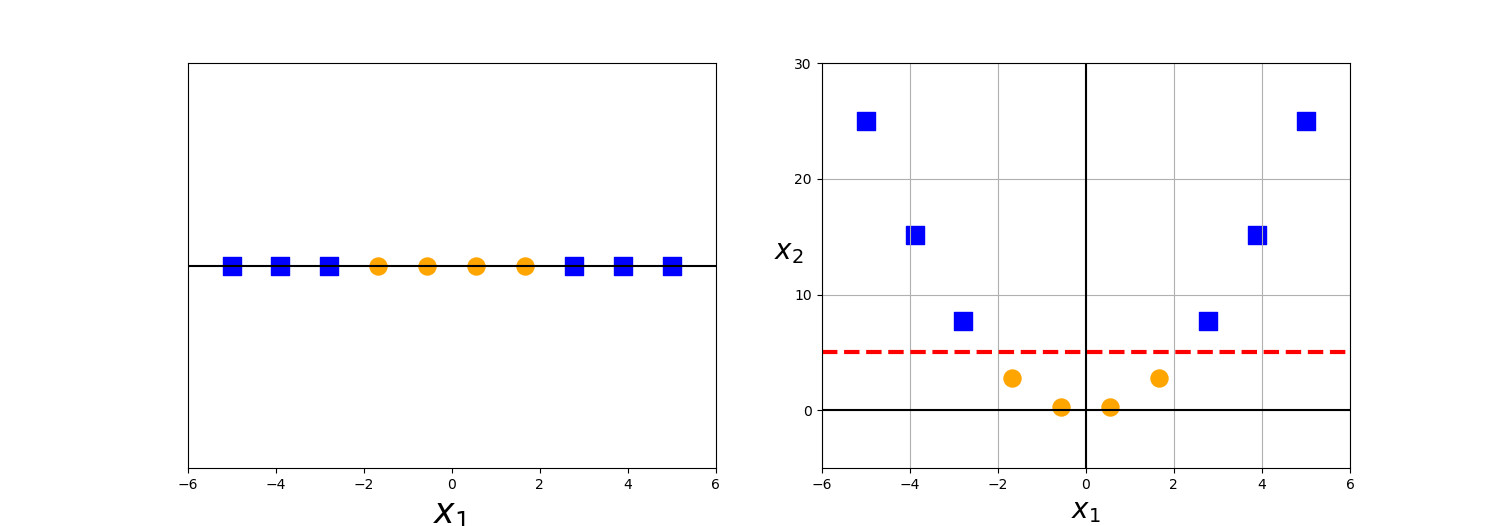
\includegraphics[width=15cm]{example}
      
        \caption{An example of a kernel transformation }        
                      
        \label{fig:example}
    \end{figure}

Some observations are summarized below:

\begin{itemize}  
\item For any given $c$, as $\sigma \to \infty$ the resulting classifier behaves like a linear classifier. Figure~\ref{fig:rbf} (e-g) shows this effect as the classification boundaries become more and more linear as $\sigma$ is increased.
\item Under-fitting (all the data points are assigned the majority class) seems to occur in cases where $\sigma$ is fixed and $c \to 0$ or $\sigma \to 0$ and $c$ is fixed to a small value. Figure~\ref{fig:rbf} (a) illustrates a case of underfitting with a small $c$ and fixed $\sigma$.
\item Over-fitting (areas around the training data points of the minority class are classified as this class while the rest is classified as the majority class) occurs when $\sigma \to 0$ and $c$ is fixed to a large value. This case is illustrated in Figure~\ref{fig:rbf} (e).

\end{itemize}
Finally, Figure~\ref{fig:compare} shows the result of applying a linear and a Gaussian kernel for the same set of training data points. Clearly, the Gaussian kernel performs better since it is able to produce non-linear decision boundaries. As previously mentioned, by mapping the data points into a high dimensional space the model becomes non linear and is able to capture more complex relationships between the data.

\begin{figure*}
 %first row: 3 subfigures
\begin{subfigure}{0.3\textwidth}
   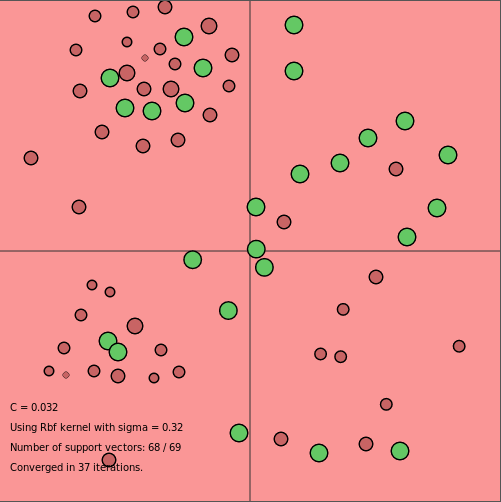
\includegraphics[width=\linewidth]{c=0032_s=032}
   \caption{$c=0.032, s=0.32$} \label{fig:x_a}
\end{subfigure}
\hspace*{\fill}
\begin{subfigure}{0.3\textwidth}
   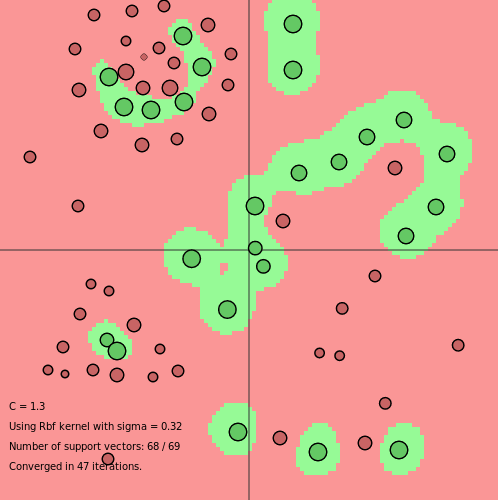
\includegraphics[width=\linewidth]{c=13_s=032}
   \caption{$c=1.3, s=0.32$} \label{fig:x_b}
\end{subfigure}
\hspace*{\fill}
\begin{subfigure}{0.3\textwidth}
   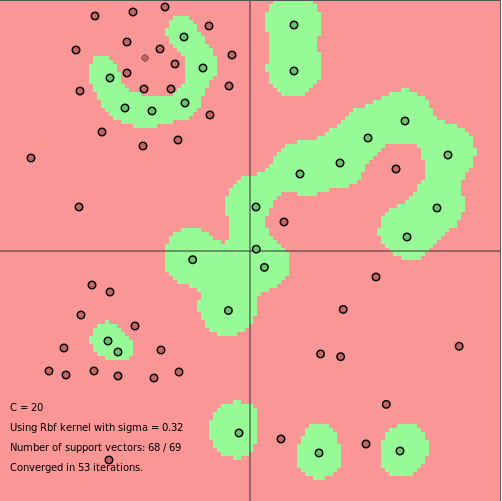
\includegraphics[width=\linewidth]{c=20_s=032}
   \caption{$c=20, s=0.32$} \label{fig:x_c}
\end{subfigure}

% 2nd row: 3 more subfigures
\bigskip
\begin{subfigure}{0.3\textwidth}
   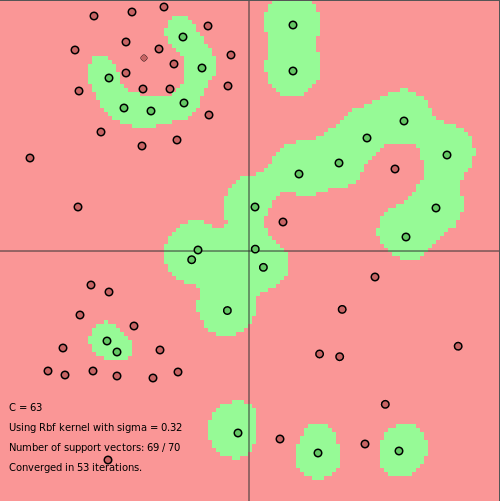
\includegraphics[width=\linewidth]{c=63_s=032}
   \caption{$c=63, s=0.32$} \label{fig:x_d}
\end{subfigure}
\hspace*{\fill}
\begin{subfigure}{0.3\textwidth}
   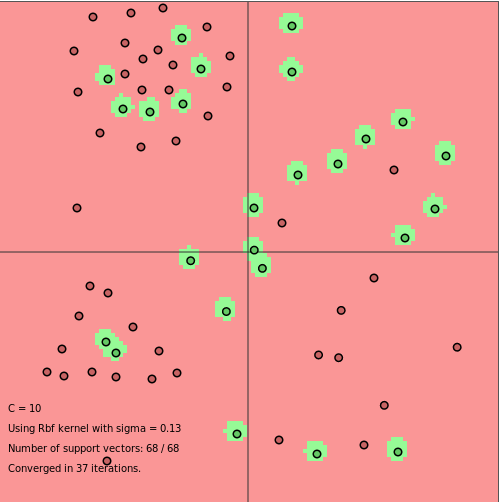
\includegraphics[width=\linewidth]{c_10_s013}
   \caption{$c=10, s=0.13$} \label{fig:x_e}
\end{subfigure}
\hspace*{\fill}
\begin{subfigure}{0.3\textwidth}
   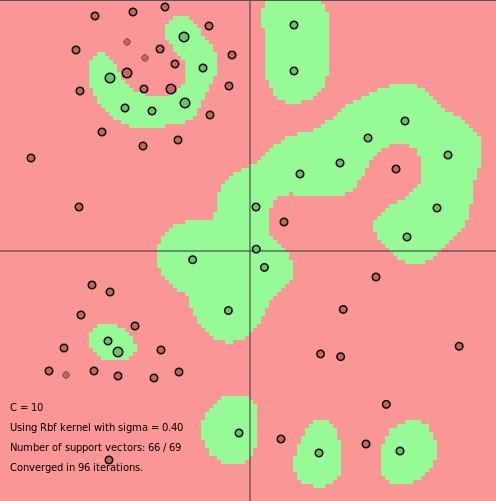
\includegraphics[width=\linewidth]{c=10_s=040}
   \caption{$c=10, s=0.43$} \label{fig:x_f}
\end{subfigure}

% 3rd row: just 2 subfigures, centered
\bigskip
\hspace*{\fill}
\begin{subfigure}{0.3\textwidth}
   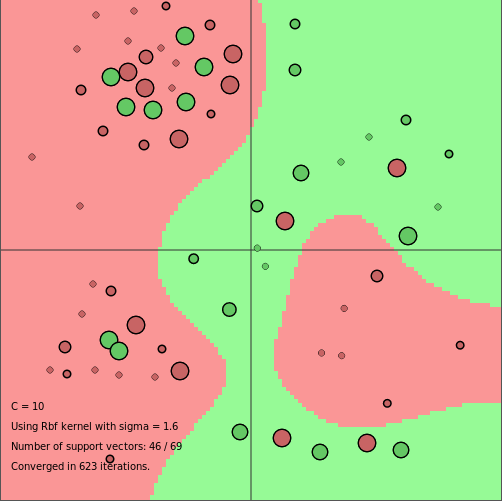
\includegraphics[width=\linewidth]{c=10_s=16}
   \caption{$c=10, s=1.6$} \label{fig:x_g}
\end{subfigure}%
\hspace*{0.05\textwidth}%
\begin{subfigure}{0.3\textwidth}
   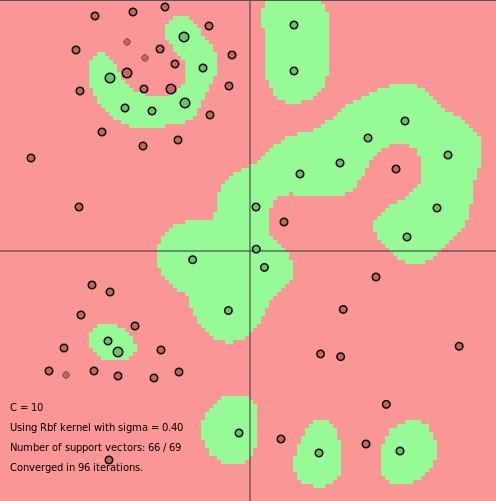
\includegraphics[width=\linewidth]{c=10_s=040}
   \caption{$c=10, s=20$} \label{fig:x_h}
\end{subfigure}
\hspace*{\fill}

\caption{Varying $c$ and $\sigma^2$ for the RBF kernel}
    \label{fig:rbf}
\end{figure*}



\begin{figure}[]

\centering
        \begin{subfigure}{0.40\linewidth}
            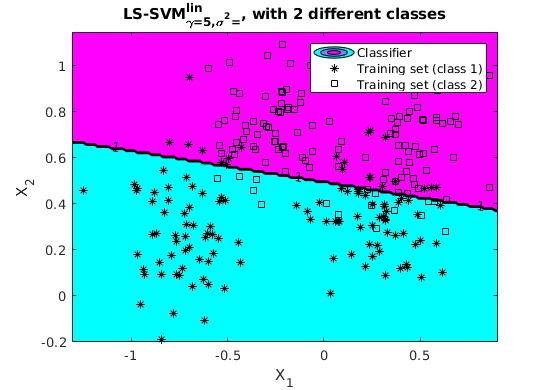
\includegraphics[width=6cm]{linear}
            \caption{Linear kernel}
        \end{subfigure}
        \begin{subfigure}{0.40\linewidth}
            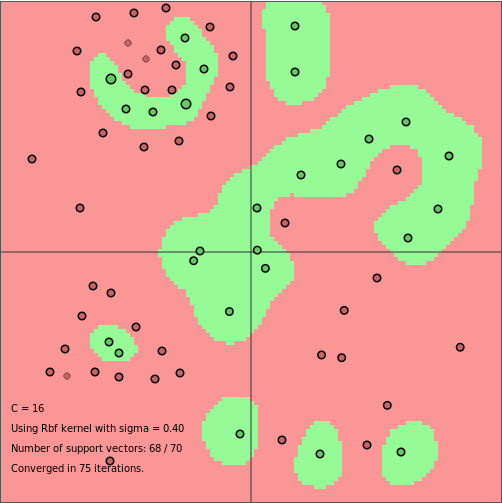
\includegraphics[width=6cm]{rbf}
            \caption{RBF kernel}
        \end{subfigure}
       

        \caption{Comparison of the decision surfaces produced by a linear (a) and an RBF (b) kernel. }        
        
              
        \label{fig:compare}
    \end{figure}


\subsection{
Least-squares support vector machine classifier}\label{hyperparameters}

\subsubsection{
Influence of hyperparameters and kernel parameters}

In this exercise, the objective is to classify the Iris dataset using a LS-SVM and explore the effect of using different kernel functions. In the LS-SVM formulation for classification the objective function becomes:


\begin{equation}
\min\limits_{w,b,e} J(w,b,e) = \frac{1}{2}w^Tw + \gamma \sum_{k=1}^{N}{e_k}^2
\end{equation}
subject to
\begin{equation*}
\begin{cases}
\begin{aligned}
  y_k[w^T\phi(x_k)+b] = 1-{e_k}, k=1,...,N \\
\end{aligned}
\end{cases}
\end{equation*}
The main difference of a LS-SVM classifier with the original SVM classifier is the use of an equality constraint instead of an inequality constraint and the use of a squared loss for the error variable $e_k$. The role of $e_k$ is similar to the role of $\xi$ in the original formulation since it defines the allowed error for the target value 1.0 (1.0 was a threshold value in the general case but here it is a target value). The advantage of this modification is that it greatly simplifies the problem which can be now solved in the dual form as a linear KKT system. An important different is that the sparsity property is lost, which means that the every data point can be considered as a support vector and $a_k=\gamma e_k$ holds for every training point $k$. The last observation leads to the conclusion that the distribution of $a_k$ variables is similar to the distribution of errors. Moreover, there is an interpretation of how relevant a data point is towards the construction of the decision boundary. All the data points are contributing to the final solution, with points that have a large $|a_k|$ being close to the decision boundary. 


The training set consists of a set of 100 data points $\{x_k,y_k\}^{100}_{k=1}$ with input data $x_k \in \mathcal{R}^2 $ and output data $y_k \in \mathcal{R} $. The test set consists of 10 different data points. For degree-d polynomials, the polynomial kernel is defined as:


\begin{equation}
K(x,x_k) = (x^Tx_k +\tau)^d
\end{equation}
where $d$ defines the degree of the polynomial kernel. According to the Mercer theorem, the only condition for the Kernel function $K$ is that it should be positive semi-definite. In that case, the convex nature of the dual SVM formulation problem guarantees that the solution found is going to be a global solution. The Mercer condition holds for all $\sigma$ values in the RBF kernel as it is expressed in equation 5 and for positive $\tau$ values in the polynomial kernel as described in equation 7. As most practical questions in machine learning, the choice of the kernel parameters is data dependent. The typical procedure is to first train a linear kernel first and observe if performance is improved by using non linear kernels. 
The degree parameter controls the flexibility of the decision boundary. Higher degree kernels yield a more flexible decision boundary but also increase the risk of overfitting. As more and more parameters are added to the model, the complexity increases which in turn leads to models of low bias but high variance.

Figure~\ref{fig:iris} (a) shows the decision boundary obtained for a linear kernel. Polynomial kernels of degree 2-4 are shown in Figure~\ref{fig:iris} (b-d). For the linear kernel, the classification error is 55\% (e.g. 11 out of 20 observations are misclassified). Applying a quadratic kernel significantly improves the performance as the prediction error drops to 5\%. For polynomials of degree $\geq 3$ the prediction error drops to 0. In the case of high order polynomial kernels the decision boundaries become more and more complex which may lead to overfitting. This is illustrated in Figure 6 (e) and (f) where a polynomial kernel of degree 15 and 20 are applied. The prediction errors for the 15 degree and 20 cases are 5\% and 20\% respectively. To conclude, following the Occam’s razor principle, the polynomial with the lowest degree that performs best should be chosen. In this particular example, the ideal choice would be either a quadratic or a cubic polynomial since the prediction error is already very small or zero.




    \begin{figure*}[]
        \begin{subfigure}{0.33\linewidth}
            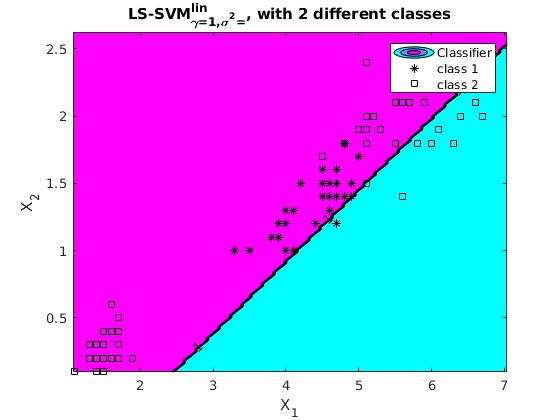
\includegraphics[width=\linewidth]{iris_linear}
            \caption{Polynomial of degree 1. Prediction error: 55\%}
        \end{subfigure}
        \begin{subfigure}{0.33\linewidth}
            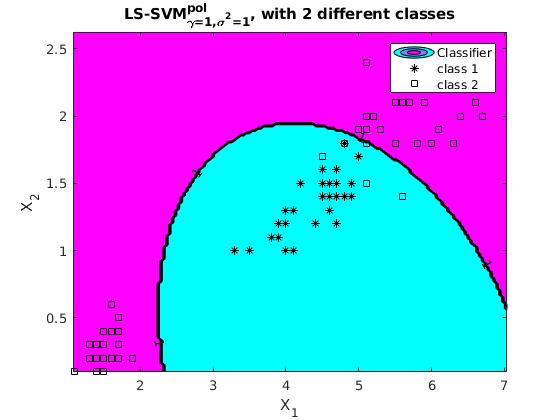
\includegraphics[width=\linewidth]{iris_degree2}
            \caption{degree 2.
Prediction error: 5\%}
        \end{subfigure}
        \begin{subfigure}{0.33\linewidth}
            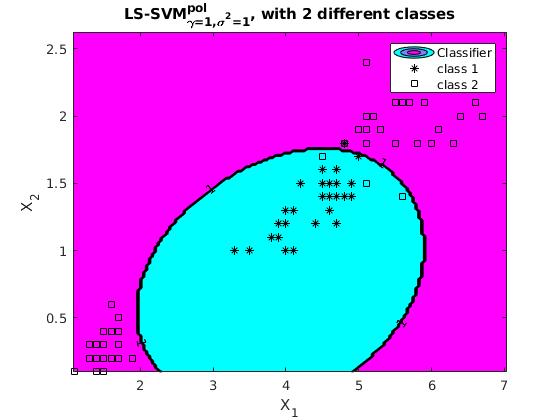
\includegraphics[width=\linewidth]{iris_degree3}
            \caption{degree 3.
Prediction error: 0\%}
        \end{subfigure}


		\begin{subfigure}{0.33\linewidth}
            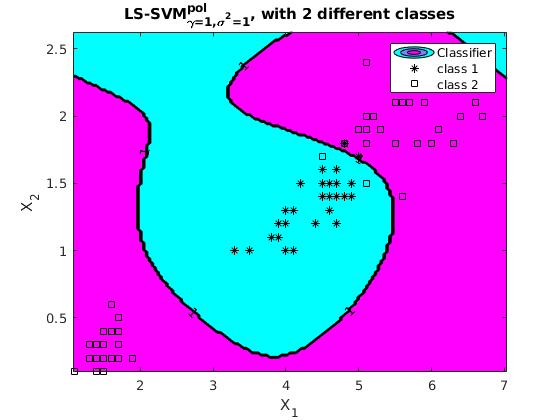
\includegraphics[width=\linewidth]{iris_degree4}
            \caption{degree 4.
Prediction error: 0\%}
        \end{subfigure}
        \begin{subfigure}{0.33\linewidth}
            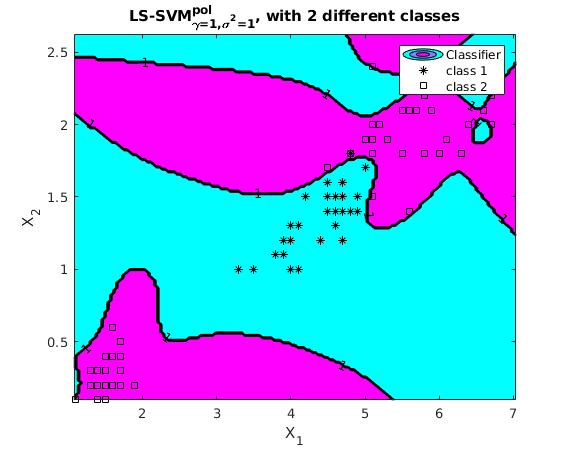
\includegraphics[width=\linewidth]{iris_degree_15}
            \caption{degree 15.
Prediction error: 5\%}
        \end{subfigure}
        \begin{subfigure}{0.33\linewidth}
            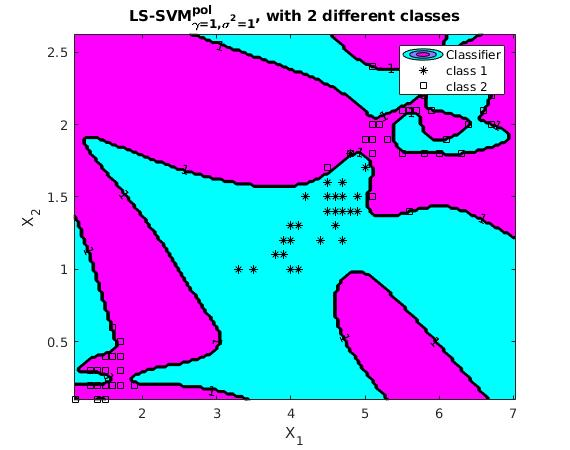
\includegraphics[width=\linewidth]{iris_degree_20}
            \caption{degree 20.
Prediction error: 20\%}

        \end{subfigure}
        
   
        \caption{ Varying the degree of the polynomial kernel.}        
        \label{fig:iris}
  \end{figure*}
  \begin{figure}[]
			\centering
            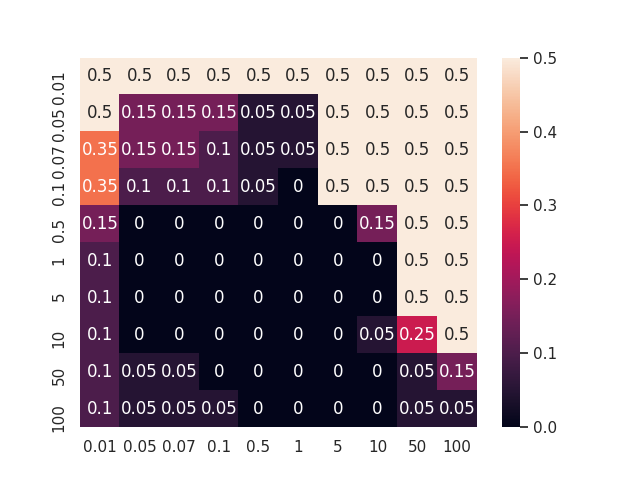
\includegraphics[width=7cm]{cgama}
      
        \caption{ Prediction error on the test set is measured for a different range of values for $\sigma^2$ (x-axis) and $\gamma$ (y-axis).  }        
        
              
        \label{fig:cgama}
    \end{figure}
    
     \begin{figure*}[]
        \begin{subfigure}{0.50\linewidth}
            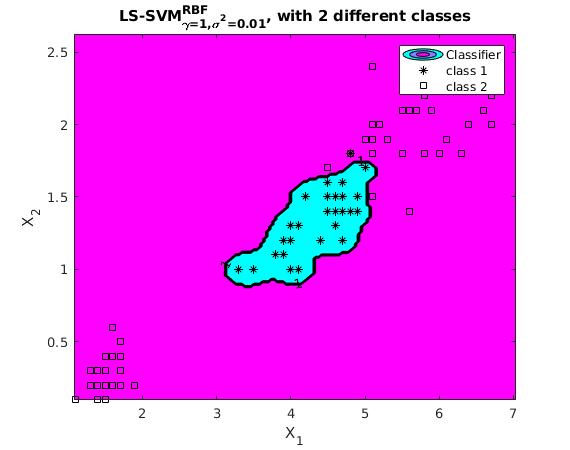
\includegraphics[width=7cm]{RBFgam1sig001}
            \caption{$\gamma=1, \sigma=0.01$}
        \end{subfigure}
        \begin{subfigure}{0.50\linewidth}
            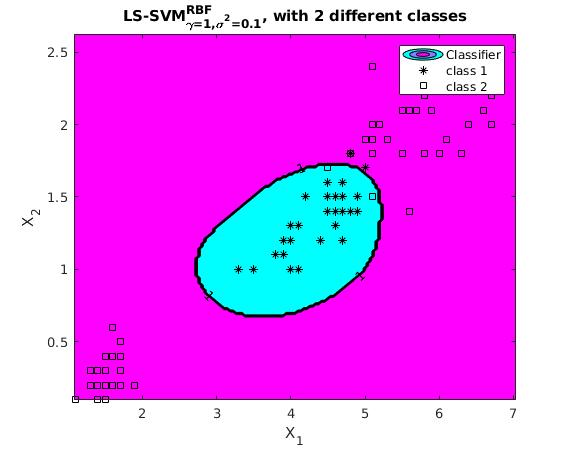
\includegraphics[width=7cm]{RBFgam1sig01}
            \caption{$\gamma=1, \sigma=0.1$}
        \end{subfigure}
        \begin{subfigure}{0.50\linewidth}
            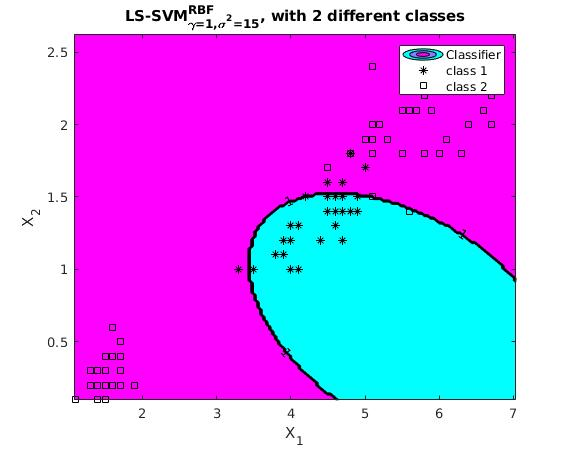
\includegraphics[width=7cm]{RBFgam1sig15}
            \caption{$\gamma=1, \sigma=15$}
        \end{subfigure}
           \begin{subfigure}{0.50\linewidth}
            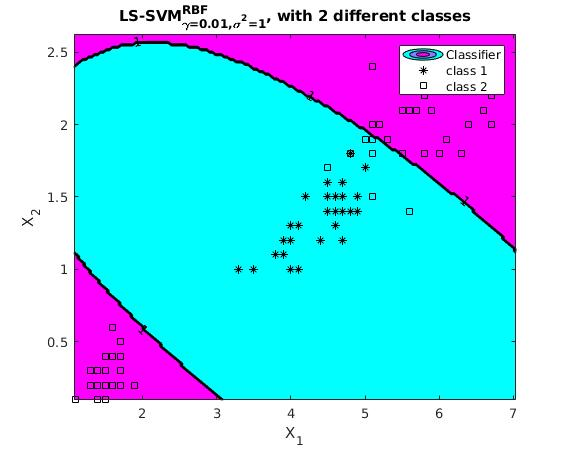
\includegraphics[width=7cm]{RBFsigma1gamma001}
            \caption{$\gamma=0.01, \sigma=1$}
        \end{subfigure}
   
        \caption{Varying $\sigma^2$ and $\gamma$ parameters in the RBF kernel. In (a) the decision boundary is centered around the points of one class which impacts the generalization ability of the classifier.  }                 
        
        \label{fig:irisrbf}
    \end{figure*}

The  effect of the parameter $\sigma^2$ was discussed in detail in the previous section. An overestimated value value for $\sigma^2$ raises the prediction error since the exponential in equation 5 will behave almost linearly and the higher-dimensional projection will lose its non-linear discriminative power. On the other hand, if underestimated, the decision boundary will become highly sensitive to noise as the model will start to overfit the data.
A grid search is performed in order to estimated the optimal values for the parameters $\gamma=$ and $\sigma^2$. Values for parameters $\gamma=$ and $\sigma^2$ are varied from 0.01 to 100 and performance on the test set is assessed and presented in Figure~\ref{fig:cgama}. The optimal values are where the prediction error is close to 0. For $\sigma^2 \in [0.05,5] $, the parameter $\gamma$ can be set to $\gamma \in [0.5,10] $ and achieve an accurate classification result with a prediction error of 0. Another possible range of values is $\sigma^2 \in [0.5,5], \gamma \in [50,100]$. In the next subsection, automated tuning algorithms for hyperparameter optimization are explored.

 
\subsubsection{Tuning parameters using validation}


In the previous question, it was shown that the performance of the solution provided by a LS-SVM classifier depends on the choice of both the parameters related to the kernel function and the $\gamma$ parameter. The parameters related to the kernel function are $d$ in equation 7 and $\sigma$ in equation 5. The goal of this exercise is to examine the efficiency and measure the performance of three different automatic tuning methods that split the raining data into a training and a validation set. Figure~\ref{fig:val} shows the contour plots that describe the performance for each one of the three methods.

\textbf{Random Split} Random Split is the simplest approach to fine-tune different parameters. The training dataset is randomly split into a training and a validation set and the model is evaluated in the latter.
Since the validation set includes data independent of that used for training, the performance of the validation set reflects the generalization ability of the model and the choice of different parameters can experimentally be tested. The validation set should not be confused with the test set which is meant to assess the performance of a fully-specified model. The error on the test set provides an unbiased estimate of the generalization error, assuming that the test set is representative of the population and follows the same probability distribution as the training set. The main problem with the random split method is that it does not exploit the full set of data to train the model which may be problematic in cases where the size of the available data is small. The generalization error will depend on the split and different validation splits may give a different generalization errors. This means that the error estimates will be highly biased, resulting in a possibly large difference between the true test error and the estimated test error. The model also becomes very sensitive to the particular choice of data over which it is evaluated. 

\textbf{K-fold Cross Validation} In $k$-fold cross validation, the original data is randomly partitioned into $k$ subsets of equal size. A single subset is used as a validation set and the model is trained on the remaining $k-1$ subsets. This process is repeated $k$ times, with a different $k$ subset used as a validation set each time. The obtained $k$ results are averaged and a single estimation is produced to evaluate the performance. The $k$-fold cross validation method tries to overcome the bias induced by the random split method. If the mean performance is satisfying this means that the model gives low error on average, ensuring that the model's notions about the data should be accurate. On the other hand, examining the standard deviation of the errors can provide an insight about the model's variance. If the standard deviation of the errors is high, this means that the model's performance varies a lot with the different splits. The main advantage of this method mainly comes from using the whole training set, providing a statistical generalization of the the random split method.

The number of folds should allow the size of each of the validation sets to be large enough to accurately reflect the population. Some observations on the size of $k$ are summarized below:

\begin{itemize}

\item A large value of $k$ will result in a small bias of the error estimates and a higher variance.
\item A small $k$ will result in a high bias in the error estimates and in a lower variance


\end{itemize}


\textbf{Leave-one-out validation} Leave-one-out cross-validation is $k$-fold cross validation applied to its logical extreme, with the parameter $k$ being equal to the number of available training instances $N$. The model is trained $N$ separate times on all the available data except one observation which is used for test. The performance is estimated by averaging the errors and models are evaluated the same way as before. It is interesting to observe that the predictions made by the models on each leave-one-out fold will have less variability since the training set is almost the same each time (the full dataset minus one data point). Intuitively, the leave-one-out method provides has a lower bias compared to $k$-fold validation since almost all of the available data are used for training.  The main drawback of this method is its computational complexity. For a training set that includes $p$ examples, leave-one-out validation requires training the model $p$ times which may become a problem for large datasets.



\begin{figure*}
 %first row: 3 subfigures
\begin{subfigure}{0.3\textwidth}
   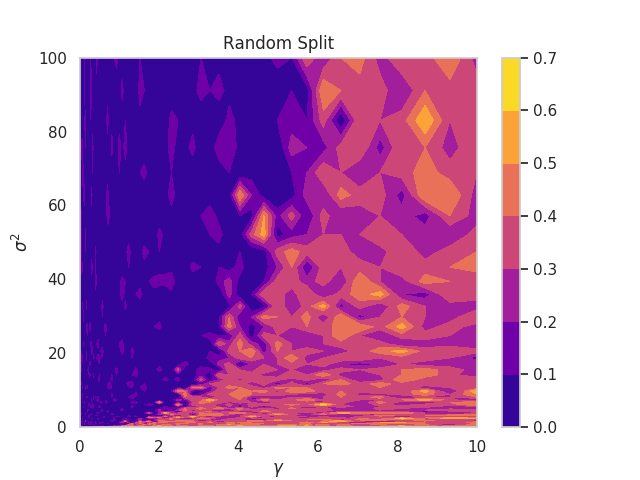
\includegraphics[width=6.6cm]{randomsplit}
   \caption{Random split} \label{fig:x_a}
\end{subfigure}
\hspace*{\fill}
\begin{subfigure}{0.3\textwidth}
   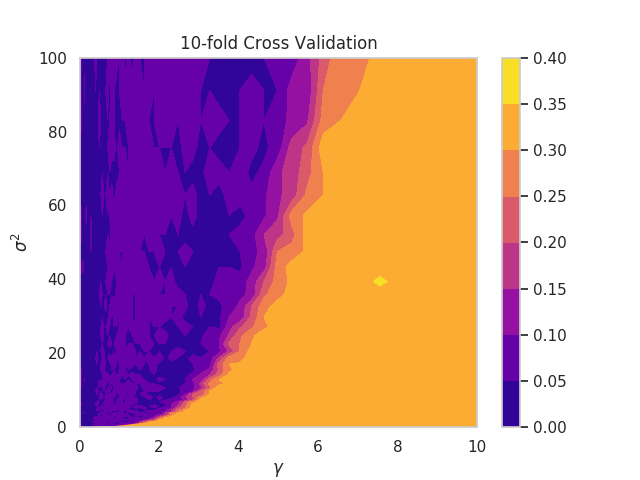
\includegraphics[width=6.6cm]{10fold}
   \caption{10-fold cross validation} \label{fig:x_b}
\end{subfigure}
\hspace*{\fill}
\begin{subfigure}{0.3\textwidth}
   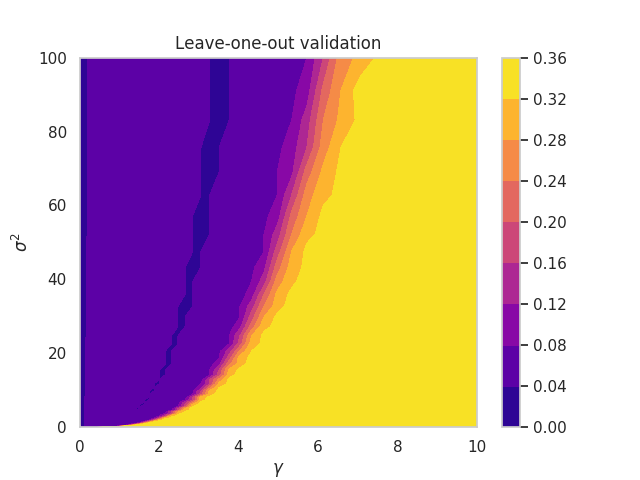
\includegraphics[width=6.6cm]{leaveone}
   \caption{leave-one-out cross validation } \label{fig:x_c}
\end{subfigure}


\caption{Visualization of the of misclassification error as a function of parameters $\sigma^2$ and $\gamma$ for Random split, 10-fold validation and leave-one-out validation }
 \label{fig:val}
\end{figure*}



\subsubsection{Automatic parameter tuning}\label{tuning}



The Nelder–Mead method is a heuristic search method that belongs to direct search optimization techniques, a class of optimization algorithms that do not use derivatives approximations but instead try to sample the objective function at a finite number of points in each iteration and decide on which actions to perform based on these values. The Gridsearch approach works very similar to the methodology applied in the previous section. All the different values for the parameters to be tuned are evaluated within a certain range and the combination that performs best is selected. The LS-SVMlab toolbox supports both the Nelder-Mead simplex and the Gridsearch algorithms \cite{tool}. First, the Coupled Simulated Annealing (CSA) algorithm determines the suitable starting points for the optimization and then these points are given to one of the optimization methods. A parallel implementation of CSA also exists, which aims to improve the speed performance. This option is denoted as directional search (RDS). Table~\ref{fig:tune1} summarizes the tuning results. The obtained hyperparameters differ every time the tuning is performed since the objective function is not convex and multiple minimum solutions may exist.

 

\begin{table*}\centering
%\ra{1.3}
\begin{tabular}{@{}rrrrrrrccrrrcrrr@{}}\toprule
& \multicolumn{4}{c}{Nelder-Mead method} & \phantom{abc}& \multicolumn{2}{c}{Gridsearch} &
\phantom{abc} \\
\cmidrule{2-5} \cmidrule{7-9} \cmidrule{10-12}
& $\gamma$ & $\sigma^2$ &     cost\% &&  $\gamma$ & $\sigma^2$ &    cost\% \\ \midrule
CSA\\
 &  6.0623 & 1.2143 &  0.0400 && 0.1930 & 5.49 & 0.04 \\

RDS\\
 &   1.4513 & 5.7490& 0.04 &&  0.0674 & 0.57 &0.03 && \\



\bottomrule
\end{tabular}
\caption{Hyperparameters tuned with Nelder-Mead method and Gridsearch for the classification task}
       \label{fig:tune1}
\end{table*}




 The LS-SVMlab toolbox integrates three optimization algorithms: Nelder-Mead algorithm, Brute force Gridsearch and Line Search.



\subsubsection{ ROC curves}

\begin{figure}[]
			\centering
            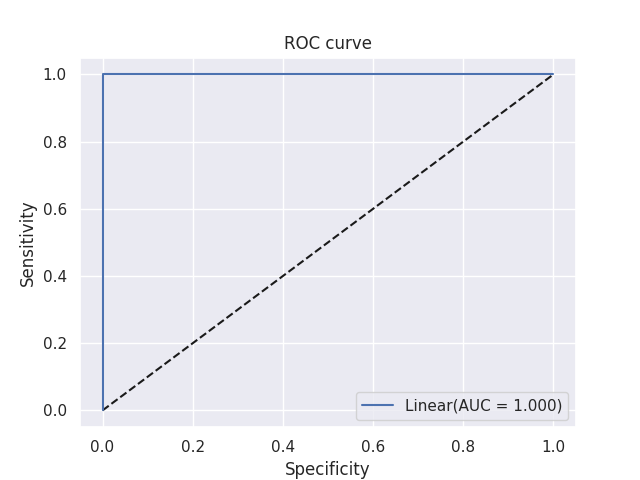
\includegraphics[width=10cm]{roc_iris}
      
        \caption{ ROC curve for the test partition of the iris dataset }        
                   
        \label{fig:roc}
    \end{figure}


The receiver operating characteristic (ROC) curves can be used to express the relationship between the sensitivity and the specificity of a classifier along different thresholds. The sensitivity (or true positive rate), plotted on the y-axis, can be described as:

\begin{equation}
TPR = \frac{TP}{TP+FN}
\end{equation}
where TP and FN (true positive and false negative) refer to the number of correctly and incorrectly classified positive instances. Therefore, sensitivity describes the fraction of correctly classified instances over the total number of positive examples. On the other hand, specificity (or false positive rate) is computed as:

\begin{equation}
FPR = \frac{TN}{TN+FP}
\end{equation}
where TN and FP (true negatives) stand for the number correctly and incorrectly classified negative instances. Specificity refers to how accurate the classifier identifies negative cases. By iteratively setting the threshold of the classifier, the curve is produced. Naturally, The area under the curve (AUC) of an ROC plot describes the quality of the classification model. If the AUC score is 1, this means that the model is able to perfectly separate the data. On the other hand, if the area equals 0.5 the classifier has no discriminative power, it simply behaves as a random classifier. The ROC curve is simply computed over the test (or validation set) and not the training set since we are interested in examining the generalization ability of the classifier. As discussed in section 1.3.2, the performance on the test set is used to provide an unbiased evaluation of the final model. 
After tuning the hyperparameters $c$ and $\sigma^2$, the ROC curve is plotted and shown in Figure~\ref{fig:roc}. The result shows that is the hyperparameters are properly selected, the obtained classifier can perfectly separate the data, having an AUC score of 1, a FPR of 0 and a TPR of 1. All of the hyperparameters described in Table~\ref{fig:tune1} produce the same result.

\subsubsection{Bayesian framework}

The Bayesian framework provides a probabilistic interpretation of the classifier. This is illustrated in Figure~\ref{fig:bay}. The uncertainty of the parameters allows to compute a probability that a point will belong either to the positive or the negative class. In this Figure it is clear that the color blue corresponds to areas that have a probability close to 0 to belong to the positive class. Conversely, areas that are depicted in yellow are related to a very high probability for the positive class. A detailed explanation of the Bayesian framework can be found in the second part of this report. 



\begin{figure}[]
			\centering
            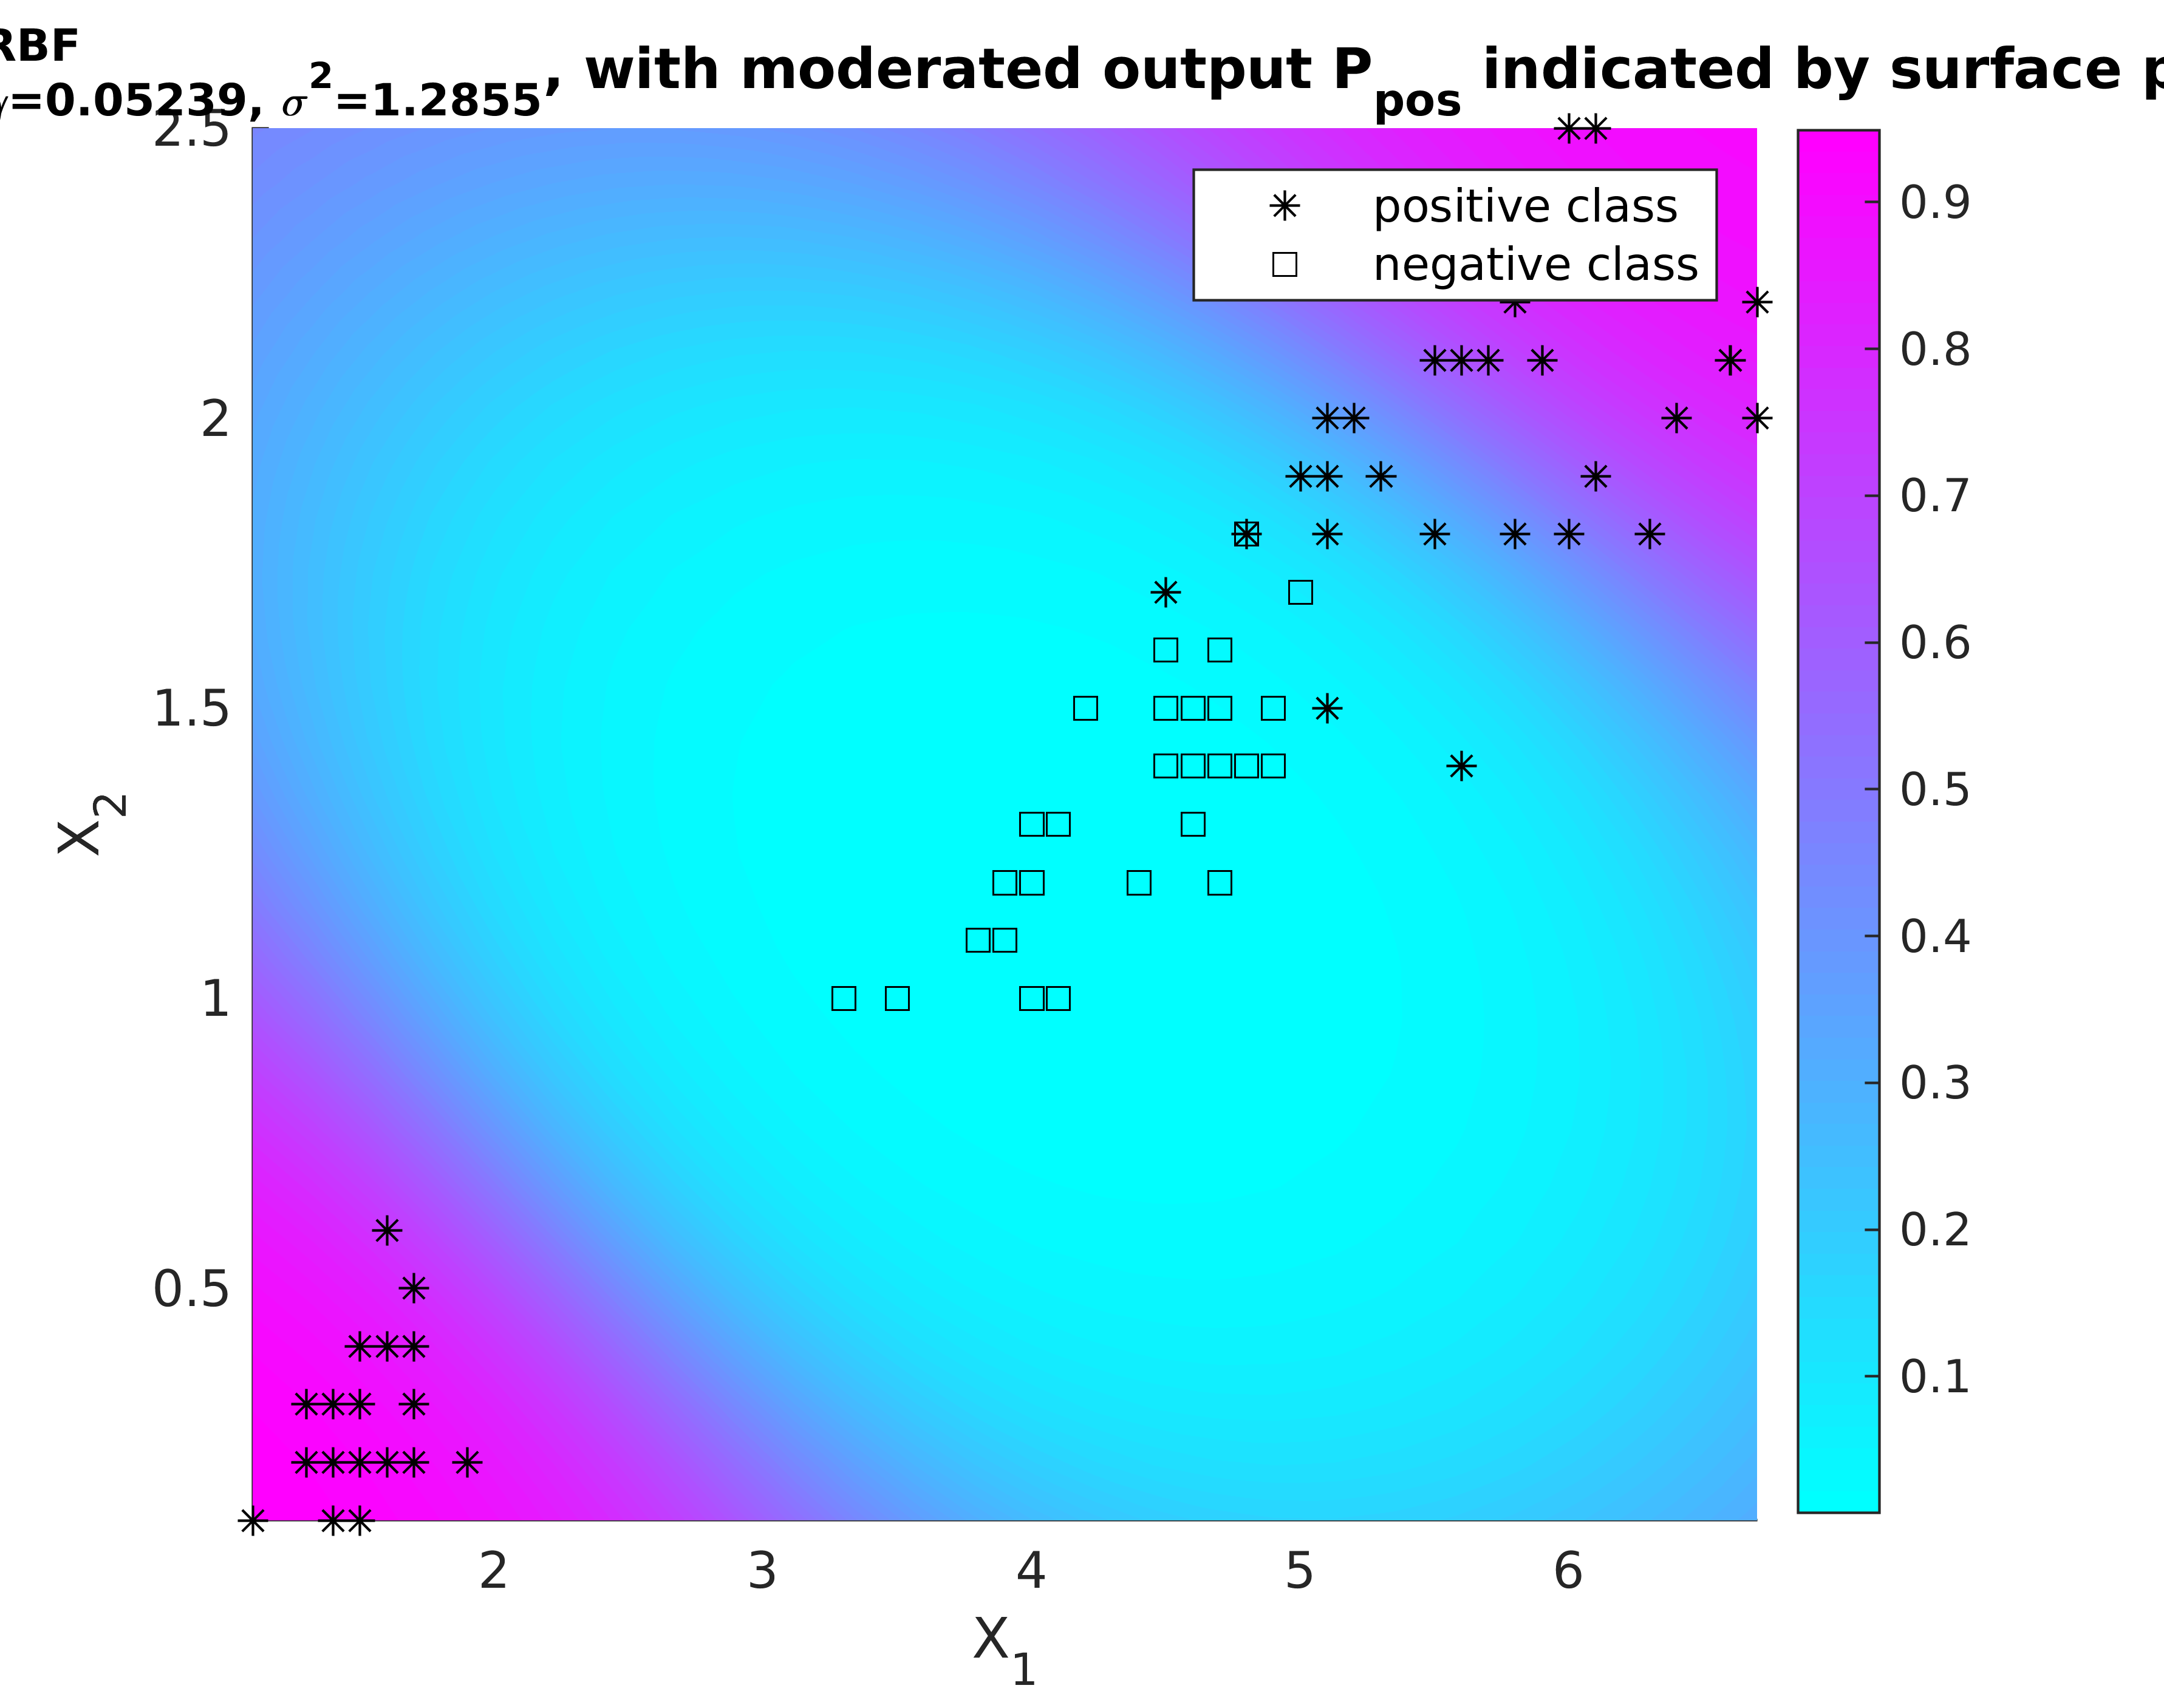
\includegraphics[width=10cm]{colormap/untitled}      
        \caption{Probabilistic interpretation of the classification boundary }                          
        \label{fig:bay}
    \end{figure}
    
\subsection{Homework Problems}
\subsubsection{Classification of the Ripley dataset}

\begin{figure*}[]
        \begin{subfigure}{0.45\linewidth}
            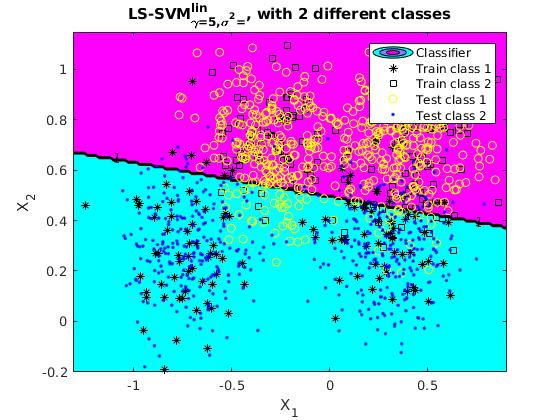
\includegraphics[width=\linewidth]{ripley_linear}
            \caption{Linear kernel}
        \end{subfigure}
        \begin{subfigure}{0.45\linewidth}
            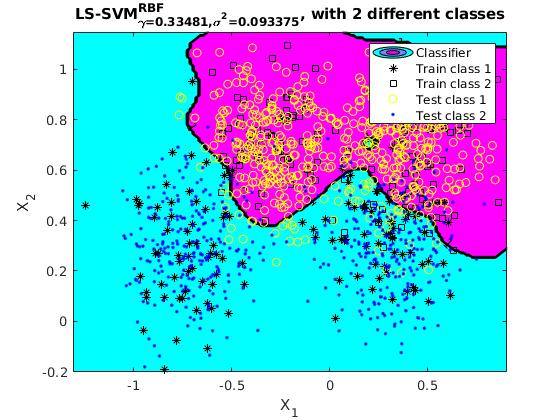
\includegraphics[width=\linewidth]{ripley_rbf}
            \caption{RBF kernel}
        \end{subfigure}
        \centering
	   \begin{subfigure}{0.45\linewidth}
            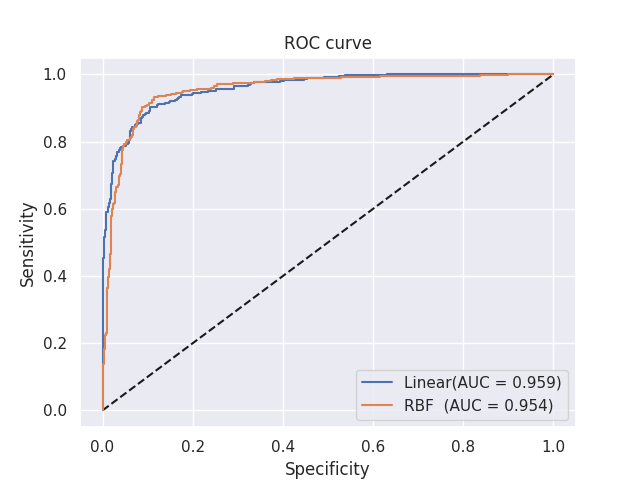
\includegraphics[width=\linewidth]{roc_ripley}
            \caption{Linear kernel}
        \end{subfigure}
         \begin{subfigure}{0.45\linewidth}
            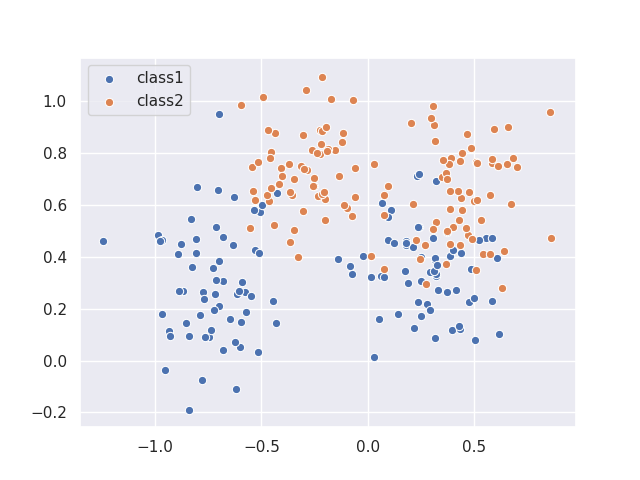
\includegraphics[width=\linewidth]{ripley}
            \caption{The Ripley dataset}
        \end{subfigure}
                   
\caption{Classifying the Ripley dataset}        
        
             
        \label{fig:ripley}
    \end{figure*}
The Ripley dataset consists of a set of input data $x_k \in \mathcal{R}^2 $ and output data $y_k \in \mathcal{R} $ with class labels $y_k \in \{-1,+1 \}$, with 250 data points intended for training and 1000 points intended for test. As illustrated in Figure~\ref{fig:ripley} (d), the two classes seem well separated from each other, although not entirely linearly separable. In the same Figure the results of applying the linear (a) and the RBF (b) kernel are also shown. The linear kernel achieves a classification accuracy of 0.89, while the RBF kernel produces a non-linear decision boundary and reaches an accuracy score of 0.90. For the RBF kernel, the hyperparamteres $c$ and $\gamma$ were tuned using the Nelder-Mead method, as described in section 1.3.3. By plotting the ROC curves in Figure~\ref{fig:ripley} (c), it is is clear that the performance of both kernels is very similar: an AUC score of 0.959 is achieved in the linear case and 0.954 in the RBF case. The conclusion is that any of the two kernels can achieve a good classification performance but since we always opt for the simplest solution the linear kernel is preferred. It is finally concluded that the performance of both models is unable to reach a better score due to the overlap of the distributions.


\subsubsection{Classification of the The Breast Cancer dataset}

\begin{figure*}[]

            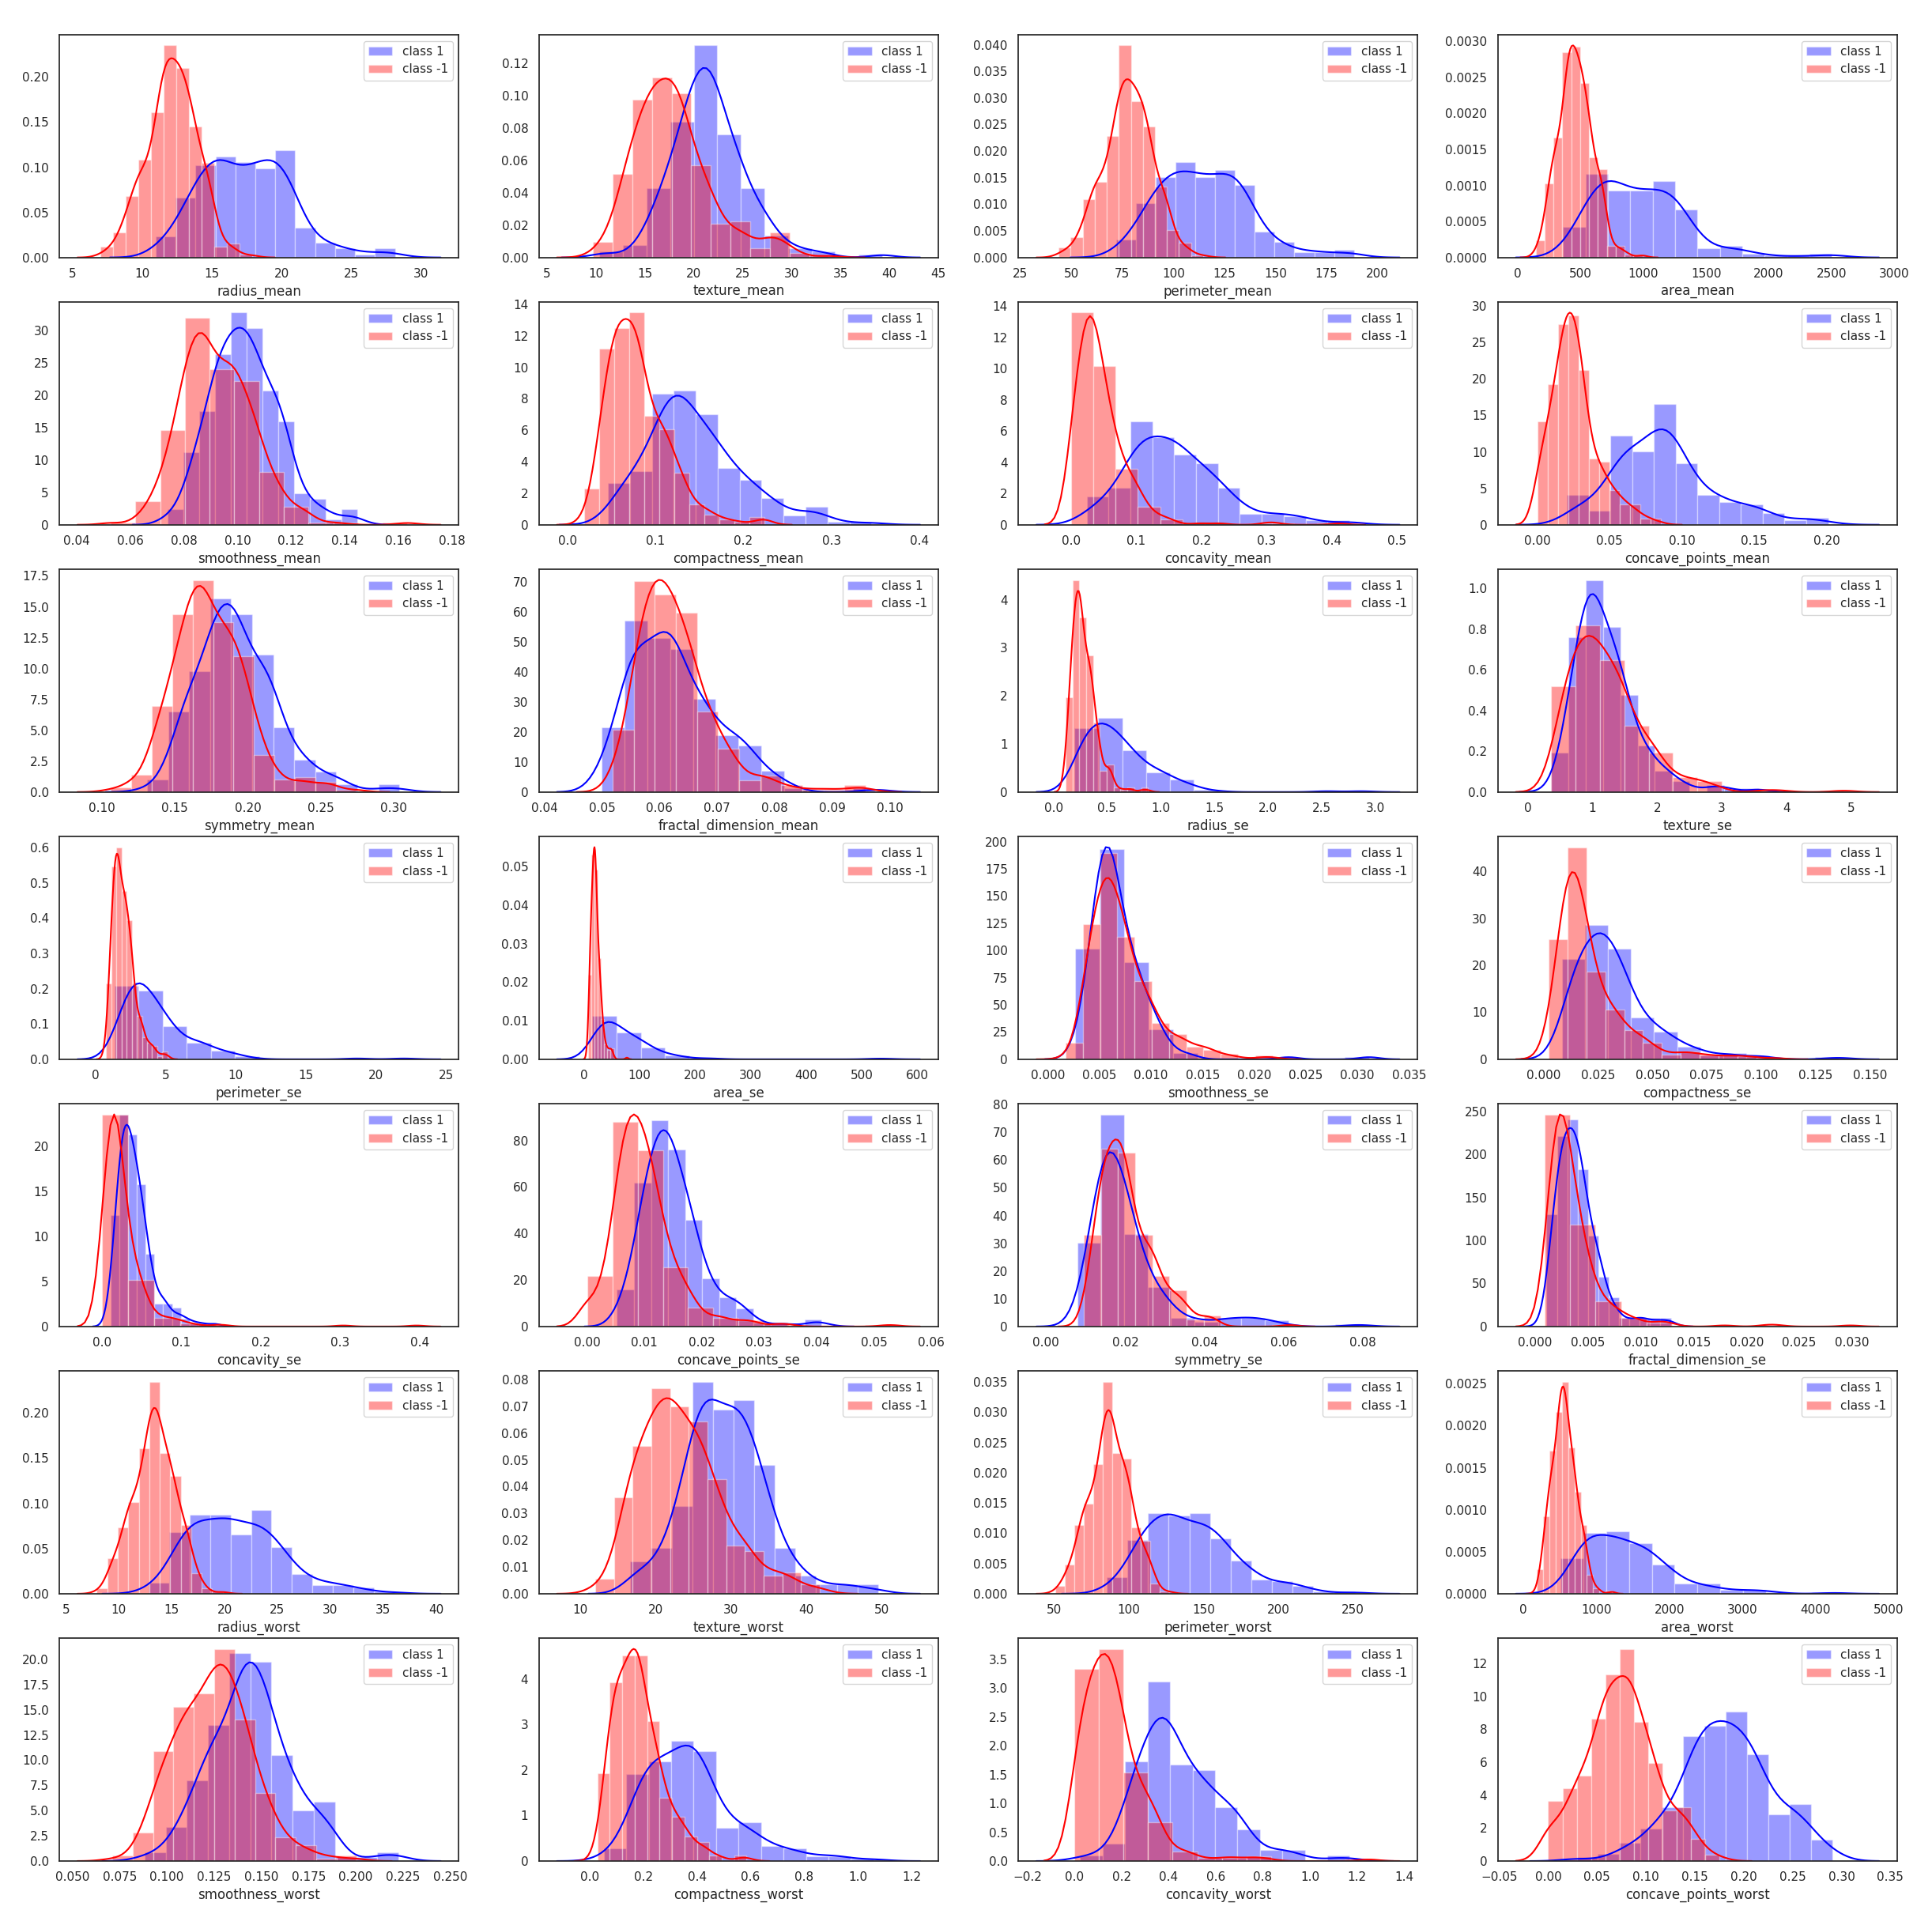
\includegraphics[width=18cm]{features_all}
      
        \caption{Distribution of features for the Breast cancer dataset }        
                   
        \label{fig:br}
    \end{figure*}
\begin{figure*}[]
        \begin{subfigure}{0.45\linewidth}
            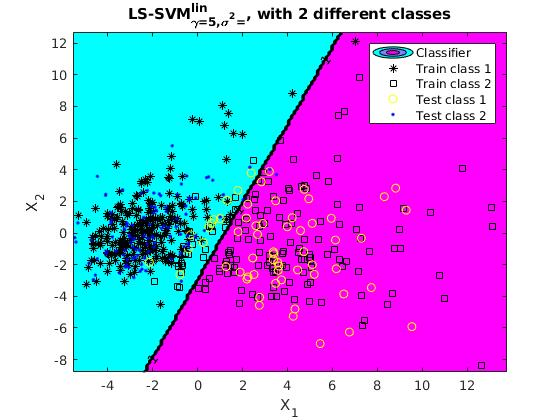
\includegraphics[width=\linewidth]{breast_linear}
            \caption{Linear kernel}
        \end{subfigure}
        \begin{subfigure}{0.45\linewidth}
            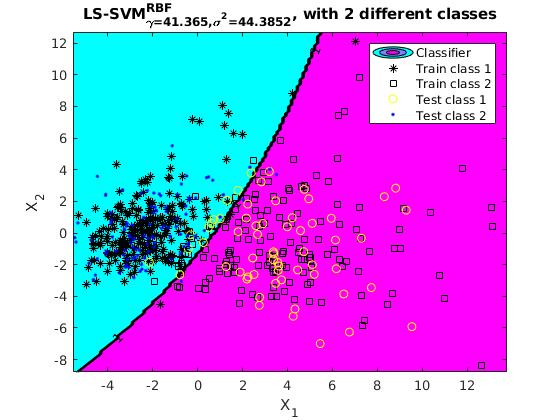
\includegraphics[width=\linewidth]{breast_rbf}
            \caption{RBF kernel}
        \end{subfigure}
        \centering
	   \begin{subfigure}{0.45\linewidth}
            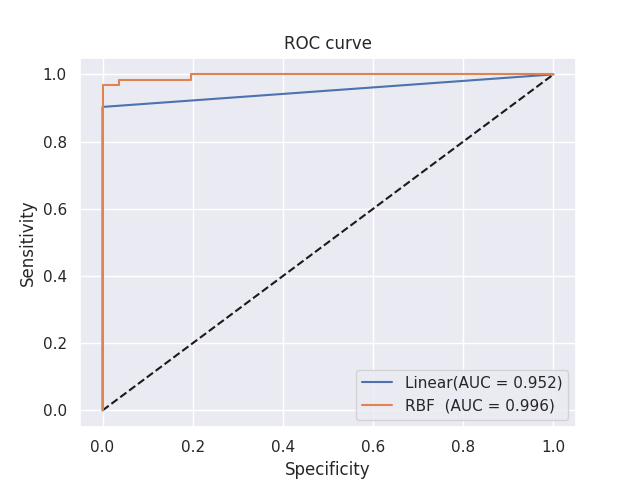
\includegraphics[width=\linewidth]{roc_breast}
            \caption{Linear kernel}
        \end{subfigure}
     
                   
\caption{Classifying the Breast cancer dataset}        
        
             
        \label{fig:brf}
    \end{figure*}


The Breast cancer dataset consists of 569 examples, with 400 intended for training and 100 for testing. The data points are composed of 30 features that describe metrics suitable for classifying cancer types as benign or malignant. The Bengin class accounts for 62.74\% of the diagnosis class while the malignant class accounts for 37.26\%. The test set follows the same class distribution as 107 out of 169 instances belong to the negative class and 69 to the positive. In Figure~\ref{fig:br}, the distributions of the values of the features are shown. Each plot corresponds to one feature. It is observed that the overlap between the two classes is smaller for some of the features (e.g. concave points worst, area worst, concave mean). Moreover, in some cases the values for class -1 are significantly larger (e.g. area se, perimeter se, readius mean, etc). Last but not least, it is shown that in some cases the variance of feature values are remarkable different (e.g. radius worst).

It will be interesting to explore whether we can reduce the dimensionality of the input data points by performing linear Principal component analysis (PCA). PCA is a dimensionality reduction technique that can be used to project the data observations into a lower dimensional space while maximizing the variance of the projected data. In short,after standardizing the input vectors, the Covariance matrix $C=\{xx^T\}$ that contains all the possible covariance pairs of the initial variables is computed. This is because the covariance matrix expresses how the variables of the observations are varying from the mean with respect to each other. The eigenvectors of this matrix show the directions where the variance is maximal and are called principal components. The amount of variance each principal component carries is expressed by the eigenvalues which can be used to rank the eigenvectors in order of significance. 



While linear PCA seems a promising solution to reduce the dimensionality while keeping the relevant information, it should be noted that it does not guarantee to always produce a better classification result. This is because the direction of maximal variance does not necessarily make the input data more separable. However, in a lot of cases applying linear PCA before training can improve the performance or simply allow to reduce the dimension of the input vector. Finally, reducing the dimension of the input vectors can be particularly useful when solving the SVM problem in its primal form where the complexity depends on the dimensionality of the data.
\begin{table}\centering
%\ra{1.3}
\begin{tabular}{@{}rrrrrrrrrrccrrrcrrr@{}}\toprule
& \multicolumn{4}{c}{Linear} & \phantom{abc}& \multicolumn{2}{c}{RBF} &
\phantom{abc} \\
%\cmidrule{2-10} \cmidrule{12-15} \cmidrule{15-20}
%PC & $2$ & $5$ &$8$ &$10$   &$15$&$30$&  cost\% &&  $\gamma$ & $\sigma^2$ &    cost\% \\ \midrule

 \textbf{2}&   &     0.9172&   &&  &0.9290 &  \\
  \textbf{5}&   &  0.9527 &   &&  &     0.9645 &  \\
   \textbf{8}&   &  \textbf{0.9645} &   &&  &   \textbf{ 0.9882} &  \\
    \textbf{10}&   & 0.9586 &   &&  &  0.9467&  \\
    \textbf{15}&   &  0.9586 &   &&  &   0.9586 &  \\
    \textbf{30}&   &  0.9527 &   &&  &  0.9467 &  \\


\bottomrule
\end{tabular}
\caption{Classification accuracy on the Breast cancer dataset after projecting the input data to 2-30 principal components}
       \label{fig:brtable}

\end{table} 
 
After scaling the data by subtracting the mean observation and by dividing with the standard deviation, a LS-SVM classifier with a linear kernel is trained by using all of the 30 features. The input data is also projected to a different number of principal components and the results and each time  are compared. Table~\ref{fig:brtable} summarizes the results. In the case where all of the 30 features are used, the classifier achieves an accuracy score of 0.9527. It is also shown that by using the first 8 principal components, the classification accuracy is improved from 0.9527 to 0.9645. Interestingly enough, by using only 5 features instead of 30 the result remains the same. The same experiment is repeated for the RBF kernel. First, $\gamma$ and $\sigma^2$ are tuned using the Nelder-Mead method and then the LS-SVM model is trained by using input vectors projected into a different number of principal components. For $\gamma=41.365$ and $\sigma^2=44.38$ and by prjojecting the input evctors to 8 principal components, the best classification score of 0.9882 is achieved. Finally, plotting the ROC curves for both kernels shows that the RBF kernel reaches a very good AUC score of 0.996, while the same score for the linear kernel is at 0.952. To conclude, in this case by performing PCA the relevant information about the features seems to be contained in the projected data and the classification accuracy is improved both in the linear and the RBF case.



\subsection{Classification of the Diabetes dataset}

\begin{figure*}[]
\centering
        \begin{subfigure}{1\linewidth}
            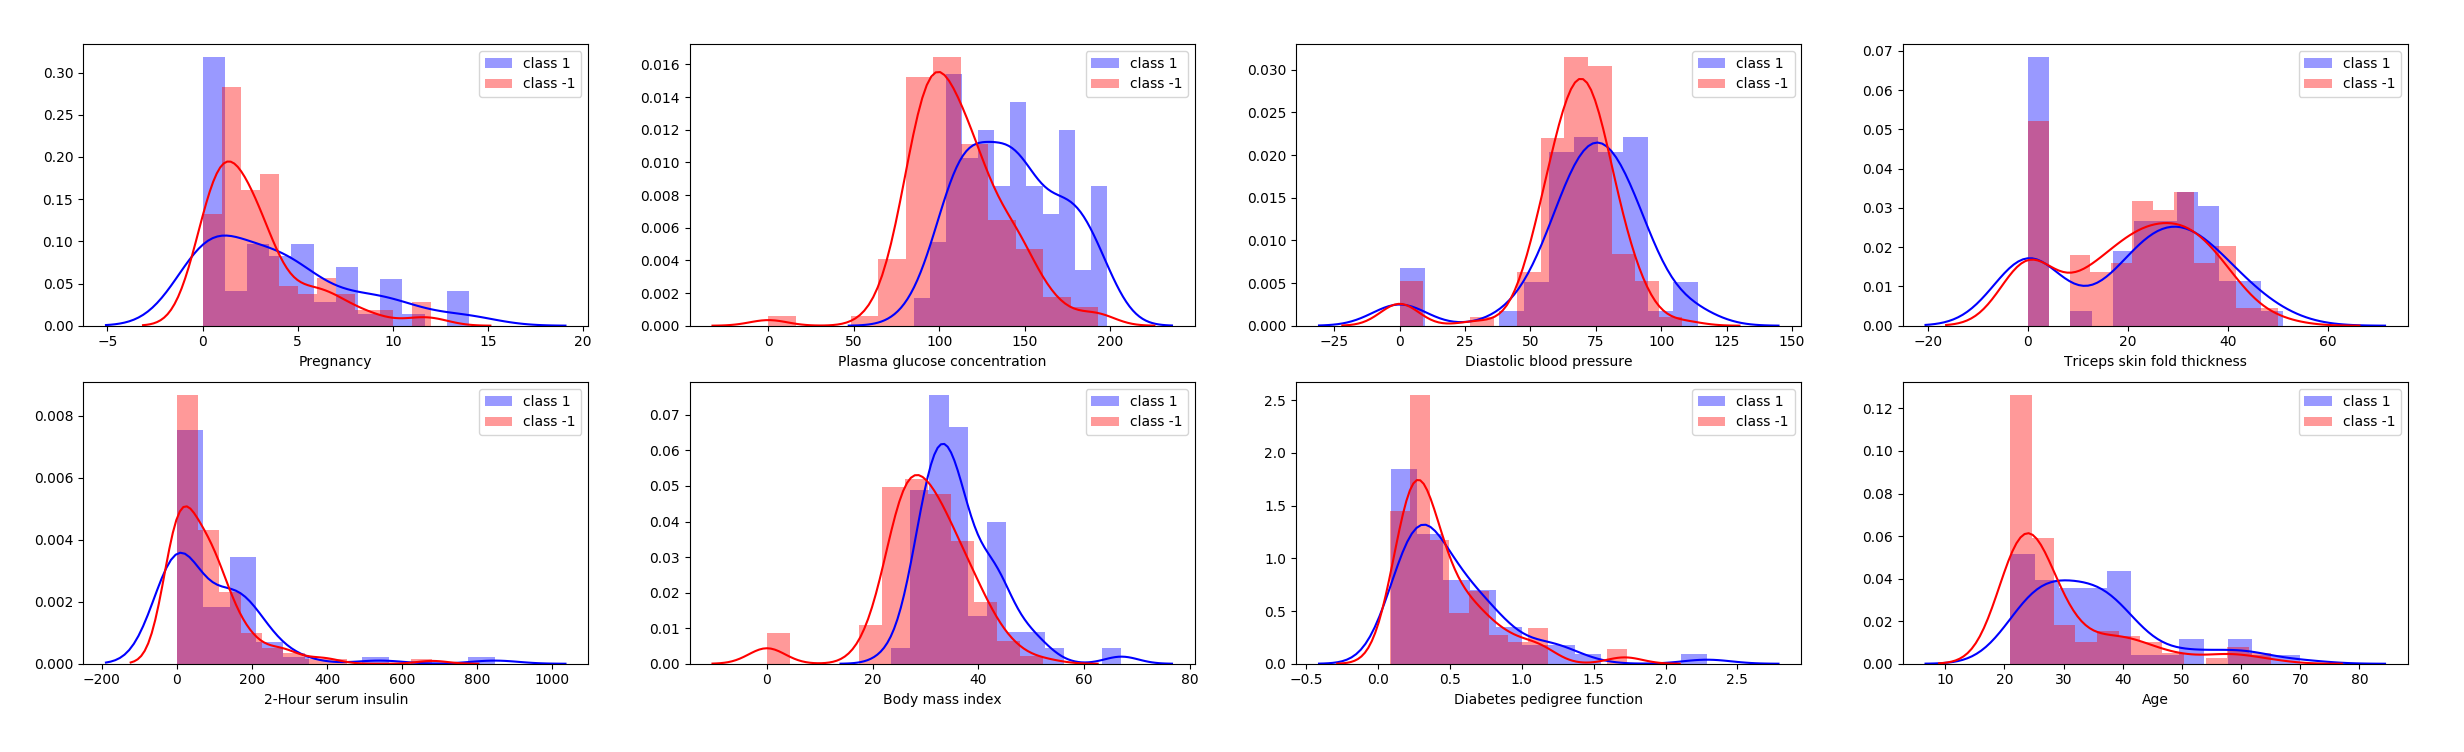
\includegraphics[width=\linewidth]{diab_train}
            \caption{train set}
        \end{subfigure}
        \begin{subfigure}{1\linewidth}
            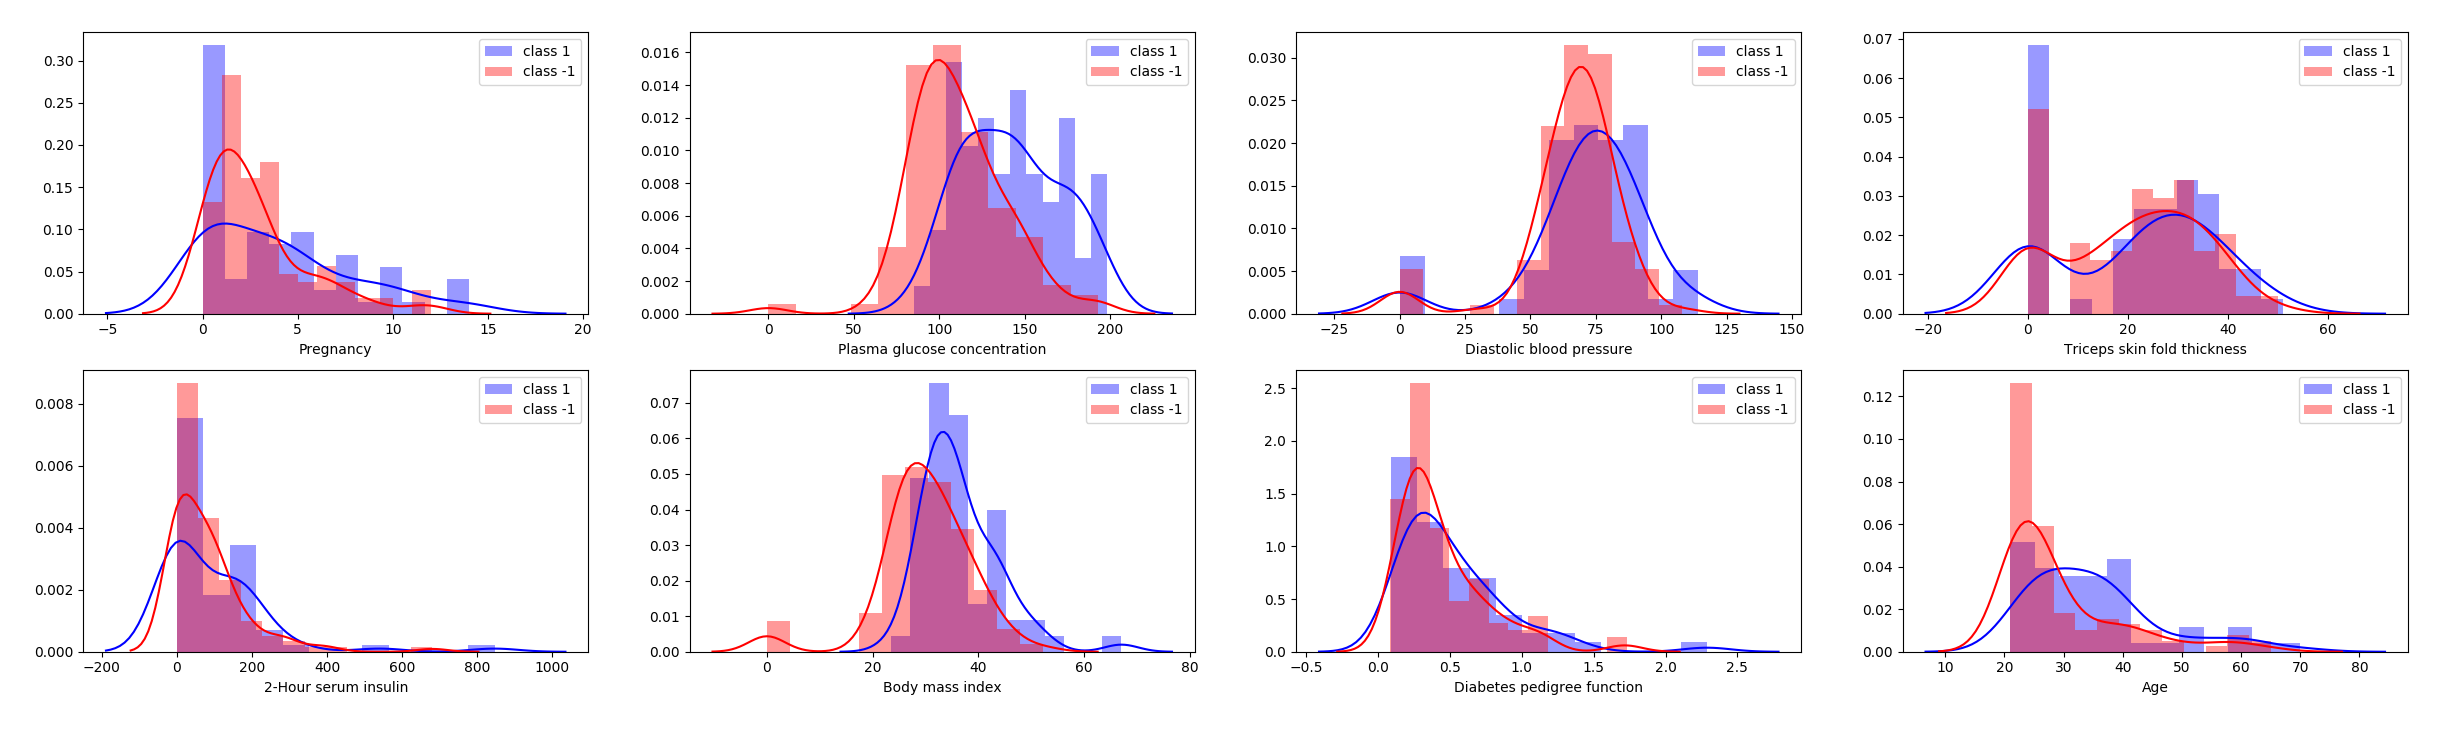
\includegraphics[width=\linewidth]{diab_test}
            \caption{test set}
        \end{subfigure}
        \centering
\caption{Distribution of features for the diabetes dataset}                 
        \label{fig:featuresdiab}
    \end{figure*}

The diabetes dataset consists of 468 instances, with 300 intended for training and 168 for testing. The data points are composed of 8 features: Plasma glucose concentration, Diastolic blood pressure, Triceps skin fold thickness, 2-Hour serum insulin, Body mass index, Diabetes pedigree function, Age and finally the number of times the patient was pregnant. Figure~\ref{fig:featuresdiab} shows the distribution of the two classes over the 8 different features. The first thing to note is that there seems to be a high overlap between the distributions of the two classes. Secondly, the feature values of the test partition seem to follow the same distribution as the values in the train partition.





\begin{table}\centering

\begin{tabular}{@{}rrrrrrrrrrccrrrcrrr@{}}\toprule
& \multicolumn{4}{c}{Linear} & \phantom{abc}& \multicolumn{2}{c}{RBF} &
\phantom{abc} \\
%\cmidrule{2-10} \cmidrule{12-15} \cmidrule{15-20}
%PC & $2$ & $5$ &$8$ &$10$   &$15$&$30$&  cost\% &&  $\gamma$ & $\sigma^2$ &    cost\% \\ \midrule

 \textbf{2}&   &    0.6310&   &&  & 0.6905 &  \\
  \textbf{3}&   &      0.6429&   &&  &  0.6845 &  \\
   \textbf{4}&   &      0.6488&   &&  & 0.6786 &  \\
   \textbf{5}&   &     0.6845&   &&  &    0.7560 &  \\
  \textbf{6}&   &  0.7143 &   &&  &        0.8036 &  \\
    \textbf{7}&   &     0.7321 &   &&  &       0.8095 &  \\
   \textbf{8}&   &  \textbf{ 0.7440} &   &&  &   \textbf{   0.8036} &  \\



\bottomrule
\end{tabular}
\caption{Classification accuracy on the Diabetes dataset after projecting the input data to 2-8 principal components}
       \label{fig:diabable}
\end{table} 

\begin{figure}[]
				\centering
            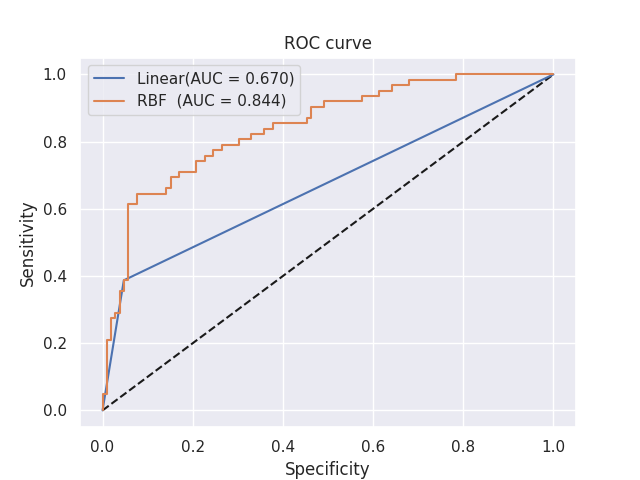
\includegraphics[width=8cm]{roc_diab}
      
        \caption{ ROC curve for the test partition of the diabetes dataset }        
                   
        \label{fig:rocdiab}
    \end{figure}


In this exercise, the same methodology as before is followed: First the data points are scaled by subtracting the mean observation and dividing with the standard deviation. Then, a LS-SVM classifier is trained by using all of the 8 features. Next, the input vectors are also projected to 2-8 principal components and results are reported in terms of classification accuracy and ROC curves. Table~\ref{fig:diabable} summarizes the outcome of this experiment. It is shown that in this case PCA does not produce a better classification result, since the best accuracy score is obtained by training with all of the 8 features. For the RBF kernel the classification accuracy is 0.8036 while for the linear case the accuracy result is 0.7440. Figure~\ref{fig:rocdiab} shows the ROC curves for the linear and the RBF kernel. The linear kernel reaches an AUC score of 0.670, while the RBF kernel performs better having an AUC score of 0.844. To conclude, the result is not as satisfying as with the previous two datasets but this is mainly attributed to the fact that there is a high overlap between the values of the available features. 




\clearpage
\section{Exercise Session 2}

The support vector machine methodology can be extended to solve linear and nonlinear function estimation problems. In the case of $N$ training data $x_k \in R^D$ and output values $y_k \in R$ the regression model takes the form: 
\begin{equation}
f(x)=w^T\phi(x)+b
\end{equation}
where $\phi(.) $ a mapping to a feature space $R^D \rightarrow R^{nD}$. As with the formulation of the problem for the classification case, the feature space can be infinite dimensional and is not explicitly defined.
The choice of loss function that evaluates how far are the predicted values $f(x)$ from the real output values $y$ is particularly important. Vapnik's $\epsilon$-sensitive loss function is a common choice:


\begin{equation}
|y-f(x)|_{\epsilon} = \begin{cases}
0 & \text{$,|y-f(x) \leq \epsilon|$}\\
|y-f(x)-\epsilon| &\text{,otherwise}
\end{cases}
\end{equation}
This particular choice of loss function is related to the notion of an $\epsilon$-tube. While in the case of classification, the support vector machine finds the hyperplane that maximizes the margin between the two classes, in the case of regression the $\epsilon$-sensitive loss defines a tube of radius $\epsilon$. All the training data points are contained within this tube and an additional constraint is introduced so that  
$|y_k-\hat{y_k}|\leq \epsilon$ or equivalently $|y_k-w^Tx_k-b|<\epsilon$ for all the observations $k$. The optimization problem in in its primal form becomes:
\begin{equation}
\min\limits_{w,b,\xi,\xi^*} J(w,b) = \frac{1}{2}w^Tw + c \sum_{k=1}^{N}(\xi_k+\xi^*)
\end{equation}
subject to
\begin{equation*}
\begin{cases}
\begin{aligned}
  y_k[w^Tx_k+b] \leq \epsilon-\xi_k, k=1,...,N \\
   w^Tx_k+b -y_k \geq \epsilon+ {\xi_k}^{*}, k=1,...,N \\
  \xi_k,{\xi_k}^{*} \leq 0, k =1,...N
\end{aligned}
\end{cases}
\end{equation*}
Solving the problem in its dual form results in the following QP problem:

\begin{equation}
\max\limits_{\alpha,\alpha^*} = -\frac{1}{2}\sum_{k,l=1}^{N}(a_k-{a_k}^{*})(a_l-{a_l}^{*})K(x_k,x_l) -\epsilon \sum_{k,l=1}^{N}(a_k+{a_k}^{*}) + \sum_{k,l=1}^{N}y_k (a_k+{a_k}^{*})
\end{equation}
subject to
\begin{equation*}
\begin{cases}
\begin{aligned}
   \sum_{k=1}^{N}(a_k+{a_k}^{*})=0 \\
  a_k,a_k^* \in [0,c]
\end{aligned}
\end{cases}
\end{equation*}
The interpretation of the lagragian multipliers $a_k, a_k^*$ is similar to the classification case. All observations strictly inside the $\epsilon$ tube should have $a_k=0$ and $a_k^*=0$ which makes the solution sparse. If either $a_k \neq 0$ or $a_k^* \neq 0$ then the corresponding point is a support vector. The two different sets of slack variables $\xi$ and $\xi^{*}$ cover two mutually exclusive situations. If $|y-f(x_k)-\epsilon|=\xi$ then the data point $x_k$ will be located above the tube, while if $|y-f(x_k)-\epsilon|=\xi^{*}$ the data point will be located below the tube. Vapnik's insensitive loss is indeed a very clever choice of a loss function, it tends to ignore small errors while for large errors it behaves like an L1 estimator. The choice of $\epsilon$ determines which points contribute to the computation of the the loss since only the predictions that are further than $\epsilon$ from the desired output are penalized. Therefore, the value of $\epsilon$ determines the width of the tube.  A very small value for $\epsilon$ will try to limit more and more points within the tube area and the constraint of equation 11 becomes harder to satisfy. This results in the conclusion that the value for $\epsilon$ controls the sparsity of the solution, or in other words the number of the support vectors. This behavior is illustrated in detail in Figure~\ref{fig:ep} where the RBF kernel is used and $c=inf$.  Increasing the $\epsilon$ value from 0.01 to 1 results in fewer support vectors and a less accurate approximation since less points contribute to the solution. 

One can also observe that if $c=inf$ then the approximation is focused simply on minimizing the error over all the training points which is a behavior very similar to a least squares fit. Consequently, the term $c$ determines the amount up to which deviations from the desired e accuracy are tolerated and controls the smoothness of the approximation. A larger value will result in a situation where less errors are allowed and will make the function less smooth. On the other hand, a small value will put greater emphasis on the minimization of the norm $||w||$ and not the summation term in equation 12, allowing more errors and smoothing the approximation. This effect is better illustrated in Figure~\ref{fig:bound} for the RBF kernel with $e=0$. As $c$ is decreased, less emphasis is put on penalizing the deviating predictions and the approximation becomes more flat. Finally, in Figure~\ref{fig:reglin} an example is illustrated where the linear kernel is more suitable for the approximation of the particular function. It is obvious that in this case the RBF, quadratic and cubic kernels exhibit nonlinear characteristics and add more complexity that needed.

%The estimated values $f(x)$ depend on both the parameter $c$ and the value of $\epsilon$.

\begin{figure}
\centering
  \begin{subfigure}{8cm}
    \centering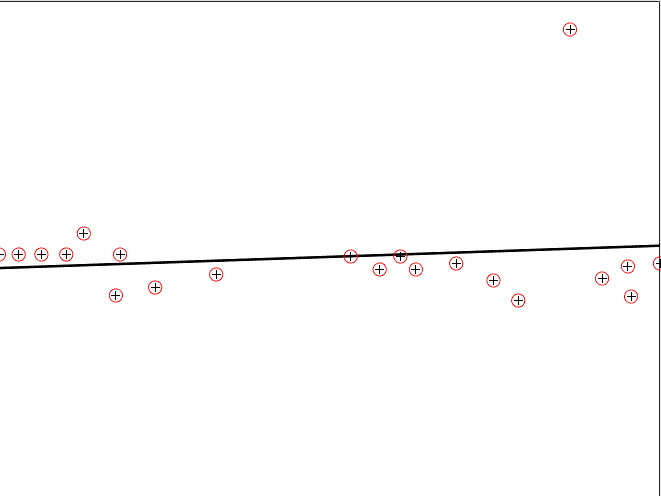
\includegraphics[width=7.8cm,frame]{1lin}
    
    \caption{linear}
  \end{subfigure}
  \begin{subfigure}{8cm}
    \centering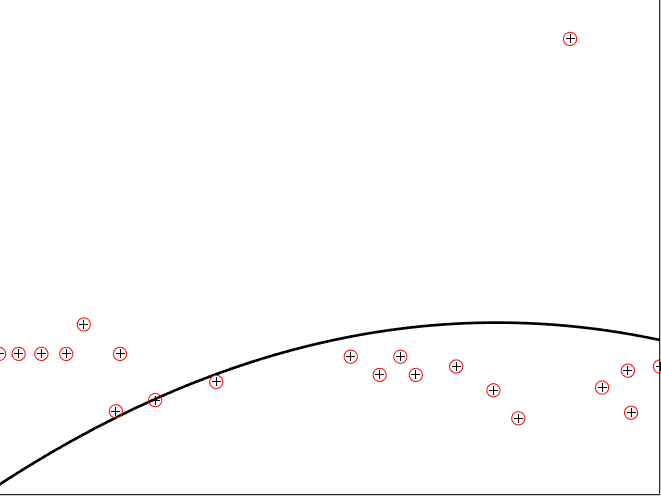
\includegraphics[width=7.8cm,frame]{1pol2}
    \caption{quadratic}
  \end{subfigure}
 \vspace{1cm}
  \begin{subfigure}{8cm}
    \centering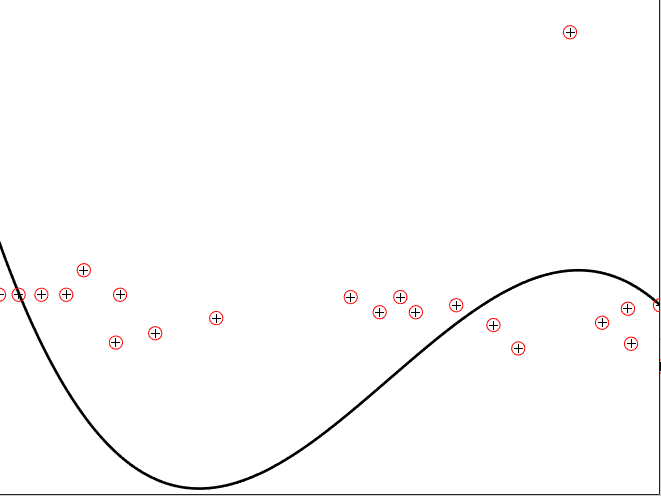
\includegraphics[width=7.8cm,frame]{1pol3}
    \caption{qubic}
  \end{subfigure}
  \begin{subfigure}{8cm}
    \centering\includegraphics[width=7.8cm,frame]{1rbf}
    \caption{RBF}
  \end{subfigure}
 
  \caption{An example where the linear kernel is the best choice for the function approximation task}
   \label{fig:reglin}
\end{figure}

\begin{figure}
\centering
  \begin{subfigure}{8cm}
    \centering\includegraphics[width=7.8cm,frame]{2b001}

    \caption{c = 0.01 }
  \end{subfigure}
  \begin{subfigure}{8cm}
    \centering\includegraphics[width=7.8cm,frame]{2b01}
    \caption{c = 0.1}
  \end{subfigure}
 \vspace{1cm}
  \begin{subfigure}{8cm}
    \centering\includegraphics[width=7.8cm,frame]{2b100}
    \caption{c = 100}
  \end{subfigure}
  \begin{subfigure}{8cm}
    \centering\includegraphics[width=7.8cm,frame]{2binf}
    \caption{c = inf}
  \end{subfigure}

  \caption{As the value of c decreases the approximation becomes more smooth and the model more sparse.}
    \label{fig:bound}
\end{figure}




\begin{figure}
\centering
  \begin{subfigure}{8cm}
    \centering\includegraphics[width=7.8cm,frame]{3e01}

\caption{$\epsilon = 0.01$, 56 support vectors }
  \end{subfigure}
  \begin{subfigure}{8cm}
    \centering\includegraphics[width=7.8cm,frame]{3e005}
\caption{$\epsilon = 0.05$, 48 support vectors}
  \end{subfigure}
 \vspace{1cm}
  \begin{subfigure}{8cm}
    \centering\includegraphics[width=7.8cm,frame]{3e02}
    \caption{$\epsilon = 0.2$, 14 support vectors}
  \end{subfigure}
  \begin{subfigure}{8cm}
    \centering\includegraphics[width=7.8cm,frame]{3e03}
\caption{$\epsilon = 0.3$, 7 support vectors}
  \end{subfigure}
    \begin{subfigure}{8cm}
    \centering\includegraphics[width=7.8cm,frame]{3e04}
\caption{$\epsilon = 0.4$, 3 support vectors}
  \end{subfigure}
    \begin{subfigure}{8cm}
    \centering\includegraphics[width=7.8cm,frame]{3e1}
\caption{$\epsilon = 1$, 2 support vectors}
  \end{subfigure}

  \caption{As the value of $\epsilon$ decreases the approximation becomes more smooth}
    \label{fig:ep}
\end{figure}




%\begin{equation}
%
%|y-f(x)|_{\epsilon} = 
%%\begin{cases}
%0,\\ if |y-f(x) \e|
%|y-f(x)-\epsilon|\\ otherwise
%
%%\end{cases}
%
%|y-f(x)|_{\epsilon} = 
%\end{equation}


\subsection{Regression of the sinc function}
\subsection{Observing the behavior of hyperparameters}
In this exercise, the objective is to approximate the function:
\begin{equation}
y = sinc (x) + \epsilon
\end{equation}
with $x \in [-10,10]$ and $\epsilon \sim N(0,1)$. We are particularly interested in solving the above problem with an LS-SVM model for function approximation using a Gaussian kernel. The optimization problem takes the following form:

\begin{equation}
\min\limits_{w,b,e} J(w,b,e) = \frac{1}{2}w^Tw + \gamma \sum_{k=1}^{N}{e_k}^2
\end{equation}
subject to
\begin{equation*}
\begin{cases}
\begin{aligned}
  y_k = w^T\phi(x_k)+b+e_k,  k=1,...,N \\

\end{aligned}
\end{cases}
\end{equation*}Similarly to the classification, an important difference of the LS-SVM formulation for function approximation is that the sparsity property is lost but the problem is greatly simplified as the solution is derived by solving a system of linear equations. In order to understand the effect of the parameters $\sigma^2$ and $\gamma$, a set of experiments was conducted in which the values of the two parameters were changed both separately and synchronously. First the value of $\gamma$ is fixed to 1000 and $\sigma^2$ is varied in the range $\sigma^2 \in [10^-3,10]$. The results of this experiment are illustrated in Figure~\ref{fig:regsig2}. Secondly, as shown in Figure~\ref{fig:regam}, $\sigma^2$ is fixed to 0.1 and $\gamma$ is varied in the range $[10^-2,10^6]$. In every case, the Mean Squared error (MSE) is used to assess the performance. 

As discussed in section \ref{hyperparameters}, the $\sigma^2$ parameter defines the influence of a single training example, with low values decreasing and high values increasing the influence zone. If $\sigma^2$ get close to $10^{-3}$, the region of influence of any of the support vectors becomes smaller, which results in overfitting (Figure~\ref{fig:regsig2}-a). Conversely, a value close to 10, makes the model too constrained and unable to capture the complexity of the function (Figure~\ref{fig:regsig2}-i). As for $\gamma$, low values close to $10^{-2}$ force the model to only minimize the norm of $||w||$ and ignore the fitness errors. This results in under-fitting since the SVM is unable to capture the relationship between the input and the outputs. Raising the value of $\gamma$ up to $10^6$ seems not to influence the prediction performance, since the model is still able to approximate the function solely based on minimizing the prediction error. However, we should be careful since very high values of the regularization parameter $c$ lead to models of high variance, which describes models of high flexibility that are more prone to overfitting. By observing the MSE for all the plotted approximations, we can  conclude that the best prediction result of 0.0117 is achieved for $\gamma=10^2$, with the worst score being 0.431 for $\gamma=10^-2.$



\begin{figure}[htb]
    \centering % <-- added

\begin{subfigure}{0.33\textwidth}
  \includegraphics[width=6.5cm]{reg/gam/1000000}
  \caption{$\gamma =10^6$}
  \label{fig:4}
\end{subfigure}\hfil % <-- added
\begin{subfigure}{0.33\textwidth}
  \includegraphics[width=6.5cm]{reg/gam/100000}
   \caption{$\gamma =10^5$}
  \label{fig:5}
\end{subfigure}\hfil % <-- added
\begin{subfigure}{0.33\textwidth}
  \includegraphics[width=6.5cm]{reg/gam/10000}
    \caption{$\gamma =10^4$}
  \label{fig:6}
\end{subfigure}

\begin{subfigure}{0.33\textwidth}
  \includegraphics[width=6.5cm]{reg/gam/1000}
  \caption{$\gamma =10^3$}
  \label{fig:4}
\end{subfigure}\hfil % <-- added
\begin{subfigure}{0.33\textwidth}
  \includegraphics[width=6.5cm]{reg/gam/100}
  \caption{$\gamma =10^2$}
  \label{fig:5}
\end{subfigure}\hfil % <-- added
\begin{subfigure}{0.33\textwidth}
  \includegraphics[width=6.5cm]{reg/gam/10}
   \caption{$\gamma =10$}
  \label{fig:6}
\end{subfigure}
\begin{subfigure}{0.33\textwidth}
  \includegraphics[width=6.5cm]{reg/gam/1}
  \caption{$\gamma =1$}
  \label{fig:1}
\end{subfigure}\hfil % <-- added
\begin{subfigure}{0.33\textwidth}
  \includegraphics[width=6.5cm]{reg/gam/01}
  \caption{$\gamma =10^-1$}
  \label{fig:2}
\end{subfigure}\hfil % <-- added
\begin{subfigure}{0.33\textwidth}
  \includegraphics[width=6.5cm]{reg/gam/001}
  \caption{$\gamma =10^-2$}
  \label{fig:3}
\end{subfigure}

\caption{Trying different $\gamma$ values for $\sigma = 0.1$}
\label{fig:regam}
\end{figure}

\begin{figure}[htb]
    \centering % <-- added


\begin{subfigure}{0.33\textwidth}
  \includegraphics[width=6.5cm]{reg/sig/0001}
  \caption{$\sigma^2=0.001$}
  \label{fig:4}
\end{subfigure}\hfil % <-- added
\begin{subfigure}{0.33\textwidth}
  \includegraphics[width=6.5cm]{reg/sig/001}
  \caption{$\sigma^2=0.01$}
  \label{fig:5}
\end{subfigure}\hfil % <-- added
\begin{subfigure}{0.33\textwidth}
  \includegraphics[width=6.5cm]{reg/sig/01}
  \caption{$\sigma^2=0.1$}
  \label{fig:6}
\end{subfigure}



\begin{subfigure}{0.33\textwidth}
  \includegraphics[width=6.5cm]{reg/sig/02}
  \caption{$\sigma^2=0.2$}
  \label{fig:4}
\end{subfigure}\hfil % <-- added
\begin{subfigure}{0.33\textwidth}
  \includegraphics[width=6.5cm]{reg/sig/04}
  \caption{$\sigma^2=0.4$}
  \label{fig:5}
\end{subfigure}\hfil % <-- added
\begin{subfigure}{0.33\textwidth}
  \includegraphics[width=6.5cm]{reg/sig/06}
  \caption{$\sigma^2=0.6$}
  \label{fig:6}
\end{subfigure}


\begin{subfigure}{0.33\textwidth}
  \includegraphics[width=6.5cm]{reg/sig/08}
  \caption{$\sigma^2=0.8$}
  \label{fig:1}
\end{subfigure}\hfil % <-- added
\begin{subfigure}{0.33\textwidth}
  \includegraphics[width=6.5cm]{reg/sig/1}
  \caption{$\sigma^2=1$}
  \label{fig:2}
\end{subfigure}\hfil % <-- added
\begin{subfigure}{0.33\textwidth}
  \includegraphics[width=6.5cm]{reg/sig/10}
  \caption{$\sigma^2=10$}
  \label{fig:sig2}
\end{subfigure}

\caption{Trying different $\sigma^2$ values for $\gamma = 1000$}
\label{fig:regsig2}
\end{figure}


\subsection{Tuning the hyperparameters}

Since we are looking for the optimal pair of $\gamma$ and $\sigma$ values a methodology similar to the one applied in section~\ref{tuning} should be followed to properly tune these parameters. In order to examine the behavior of the Nelder-Mead simplex and the Gridsearch algorithms, the hyperparameter tuning is repeated for 100 times and aggregated statistics are reported in Table~\ref{table:tune2}. More specifically, the mean values $\mu_\gamma, \mu_{\sigma^2}$ as well as the standard deviations $\sigma_\gamma, \sigma_{\sigma^2}$ for every optimization algorithm are shown. At a first glance, it is obvious that the optimal values for $\sigma^2$ fall in a much narrower range than the values for $\gamma$. The mean value for $\gamma$ is 12335 in the Nelder-Mead case and 12450 in Gridsearch with standar deviations 29423 and 10404 respectively. Figure~\ref{fig:tune3} (a) and (c) describe this situation in further detail. While the majority of $\gamma$ values seem do be centered around a small area, in the case of Nelder-Mead they are more spread. By examining the histogram and estimated density plots of the $\sigma^2$ parameter, it is concluded that the distribution of the values produced by Gridsearch is described by two peak areas, around $\sigma^2 \in [0,0.2]$ and $[0,0.4]$. On the other hand, the Nelder-Mead algorithm seems to be focused on a smaller range and returns values centered around the mean observation of the population. Figure~\ref{fig:tune4} shows the behavior of both algorithms with respect to the Mean Squared error. From this figure it is clear that multiple combinations of $\gamma$ and $\sigma^2$ could be optimal and the choice of tuning algorithm affects the search area.

An advantage of the Nelder-Mead algorithm is its fast execution time. As far as Gridsearch is concerned, the computational cost of evaluating the function for each pair of values is parameter dependent. This means that if we want to search a large range of values this will cost extra time. The Nealder-Mead algorithm behaves in a more clever way since it explore pairs of parameters only if they lead to a solution. Additionally, since it is not a gradient-based optimization method, the risk of converging to local minima solutions is absent.



\begin{figure}
\centering
  \begin{subfigure}{8cm}
    \centering\includegraphics[width=7.8cm]{r2/gamma}

    \caption{Histogram of $\gamma$ values }
  \end{subfigure}
  \begin{subfigure}{8cm}
    \centering\includegraphics[width=7.8cm]{r2/sigma}
    \caption{Histogram of $\sigma^2$ values }
  \end{subfigure}
 \vspace{1cm}
  \begin{subfigure}{8cm}
    \centering\includegraphics[width=7.8cm]{r2/gamma_kde}
 \caption{Density estimation for $\gamma$ parameter}
  \end{subfigure}
    \begin{subfigure}{8cm}
    \centering\includegraphics[width=7.8cm]{r2/sigma_kde}
    \caption{Density estimation for $\sigma^2$ parameter}
  \end{subfigure}
\caption{Observing the distribution of the tuned parameters}
    \label{fig:tune3}
\end{figure}


\begin{figure}
\centering
  \begin{subfigure}{8cm}
    \centering\includegraphics[width=7.8cm]{r2/simplex}
   \caption{Nelder-Mead algorithm}
  \end{subfigure}
   \begin{subfigure}{8cm}
    \centering\includegraphics[width=7.8cm]{r2/gridsearch}
   \caption{Gridsearch algorithm}
  \end{subfigure}

  \caption{Kernel Density estimate}
    \label{fig:tune4}
\end{figure}

\begin{table*}\centering
%\ra{1.3}
\begin{tabular}{@{}rrrrrrrccrrrcrrr@{}}\toprule
& \multicolumn{4}{c}{Nelder-Mead method} & \phantom{abc}& \multicolumn{2}{c}{Gridsearch} &
\phantom{abc} \\
\cmidrule{2-5} \cmidrule{7-9} \cmidrule{10-12}


 &   $\mu_\gamma=12335.94$ & $\mu_{\sigma^2}= 0.21$ &  &&  $\mu_\gamma= 12450.99$ & $\mu_{\sigma^2}= 0.39$ \\\\
 
  &    $\sigma_\gamma=29423.54 $& $\sigma_{\sigma^2}= 0.12$ &&& $\sigma_\gamma=10404.12 $& $\sigma_{\sigma^2}= 0.12$ \\\\
  

\bottomrule
\end{tabular}
\caption{Hyperparameters tuned with Nelder-Mead method and Gridsearch for the function approximation task}
       \label{table:tune2}
\end{table*}

\subsection{Application of the Bayesian framework}


In a Bayesian learning setting, instead of characterizing learning by a point $w$ in the weight space, we consider a distribution on the parameter $w$. This means that we assign a probability over all the possible values of vector $w$ rather than interpreting $w$ as an individual point. We have to consider a prior distribution $p(w)$ that describes the probability of of a vector $w$ before seeing the data $D$ and a likelihood distribution $p(D|w)$ that refers to the probability of the data $D$ given the parameter vector $w$. These two distributions define the posterior distribution $p(w|D)$ as: $P(w|D)=\frac{P(D|w)P(w)}{P(D}$.
A Bayesian framework that applies this rule on three hierarchical levels of inference can be used to a) select the most suitable model $H$, b) use the principle of automatic relevance determination to do input selection based on the errors bars derived from the output. The three levels of inference are described below considering an RBF kernel with width $\sigma$:

\textbf{First level} In the first level, the primal weight space parameters $w$ and $b$ are inferred. In the case of an LS-SVM the original objective function is extended to include a second regularization hyperparameter $\mu$:

\begin{equation}
\min\limits_{w,b,e_c} J_P(w,e_c) = \mu \frac{1}{2}w^Tw + \zeta \sum_{k=1}^{N}e_{c,k}^2
\end{equation}
The posterion distribution on the unknown parameters $w,b$, given the regularization terms $\mu,\zeta$ and the model $H_\sigma$ is described as:

\begin{equation}
p(w,b|D,\mu,\zeta,H_\sigma) = \frac{p(D|w,b,\mu,\zeta,H_\sigma)}{p(D|\mu,\zeta,H_\sigma}p(w,b|\mu,\zeta,H_\sigma)
\end{equation}
The product of the last equation can be converted into a sum by taking the log in both sides of the equation. The term $\mu$ is then associated with the prior $p(w,b|\mu,\zeta,H_\sigma)$. More specifically, the value of $\mu$ determines the amount of variance of the prior distribution, with larger values putting more emphasis on minimizing the first term of equation 16 which makes the prior more peaked. Naturally, the second term of equation 16 corresponds to the likelihood distribution. By minimizing the negative logarithm of the posterior in equation 17, one can obtain the maximum posteriori solution vectors $w_{MP}$ and $b_{MP}$. The maximization of the logarithm of the posterior corresponds to the minimization of the objective function of equation 16.

\textbf{Second level} The second level of inference refers to infer the hyperparameters $\mu$ and $\zeta$. The application of Bayes rule on the posterior distribution that characterizes these parameters is the following:

\begin{equation}
p(\mu,\zeta|D,\mu,H_\sigma) = \frac{p(D|\mu,\zeta,H_\sigma)}{p(D|H_\sigma)}p(\mu,\zeta|H_\sigma)
\end{equation}
One can observe that the likelihood term $p(D|\mu,\zeta,H_\sigma)$ of equation 18 is the evidence of equation 17. Therefore, it is possible to use the expressions derived in the first level and develop analytical expressions for the posterior of this level. An independence assumption is also  made in a sense that $p(\mu,\zeta|H_\sigma) = p(\mu|H_\sigma)p(\zeta|H_\sigma)$ one can derive analytical expressions of the posterior and solve an optimization problem to determine the model $H\sigma$.
Taking the negative logarithm of the posterior distribution of equation 18 we can solve an minimization problem and obtain the maximum posteriori estimates $\mu_{MP}$ and $\zeta_{MP}$.

\textbf{Third level} The third level of inference is related to the kernel parameters and can be used for model selection. The concept is similar to the previous two levels, the distribution over all the kernel parameters can be expressed as:

\begin{equation}
p(H_\sigma|D) = \frac{p(D|H_\sigma)}{p(D)}p(H_\sigma)
\end{equation}
where $H\sigma$ refers to an RBF kernel with width $\sigma$. If we assume that all possible kernel parameters $\sigma$ are equally likely, we can consider the prior $p(H_{\sigma})$ as a uniform distribution. The likelihood $P(D|H_\sigma)$  
also appears as the evidence term of equation 18. Following the same methodology as in the previous levels, we can compute the posterior by using the likelihood $P(D|H_\sigma)$.
To summarize, every level in the Bayesian framework applies the Bayes rule in order to infer either the primal parameters (first level), the hyperparameters (second level) or the kernel parameters (third level). This is possible since the likelihood appearing in the equation of each level is the evidence term in the previous level. Finally, by maximizing the logarithm of the posterior distributions one can solve the parameters selection task as an optimization problem over these parameters. 

In order to further understand the described framework we apply it to the function of equation 14. The implemented functions available in the LS-SVMlab toolbox estimate the posterior probabilities of the tuning parameters on the three aforementioned levels. More specifically, the \textit{bay\_optimize} function is used to optimize the posterior probabilities of the model hyperparameters with respect to different levels. The \textit{bay\_lssvm} function computes the negative logarithm of the posterior in each level which describes the corresponding cost. The obtained hyperparameters for the function approximation task are $\gamma=2.11$, $\sigma^2=0.15$. These values are aligned with the parameter tuning results of the previous section. The result of applying the Bayesian framework the LS-SVM model is shown in Figure~\ref{fig:bayes}. The right side of this Figure shows the error bars which correspond to the confidence of the prediction. The black line is the predicted function while the red dotted line represents the area in which 95\% of the data resides. The estimated error bars of the points is 0.087. By plotting $-log(P(D|H_\sigma)$ in Figure~\ref{fig:bayes} (c) also shows that the optimization problem in this case is convex. It should be noted however that the problems that the Bayesian framework defines are not always convex but in many cases this is indeed the situation.


\begin{figure*}[]
        \begin{subfigure}{0.45\linewidth}
            \includegraphics[width=\linewidth]{bayesian/bayesian_regression1}
            \caption{}
        \end{subfigure}
                \begin{subfigure}{0.45\linewidth}
            \includegraphics[width=\linewidth]{bayesian/bayesian_regression2}
            \caption{}
        \end{subfigure}
                \centering
        \begin{subfigure}{0.45\linewidth}
            \includegraphics[width=\linewidth]{bayesian/bayes_opt}
            \caption{}
        \end{subfigure}
                  
\caption{Applying the Bayesian framework for the function approximation task}        
        
             
        \label{fig:bayes}
    \end{figure*}

%The main advantages of the described framework are summarized below:

\begin{itemize}

\item The complexity of the model can be controled 
\item predictive distribution of outputs
\item use prior info and and hierarchical models for hyperparameters
\end{itemize}

%

\subsection{Automatic Relevance Determination}
Automatic Relevance Determination is a method that aims to assess the relevance of the input variables. The original definition of the RBF kernel is changed so that it includes a diagonal matrix $S$. The $S$ matrix contains as many values as the dimensionality of the input space, with each one of them describing the relevance of this particular input. The algorithm starts with a $\sigma$ as a starting point. The unknown parameters of the diagonal matrix $S$ then form an optimization problem similar to the one that is solved by the third level of the Bayesian framework. In each step the input with the largest $\sigma^2$ is removed. After the execution of the algorithm, the most relevant inputs are expected to have large weights, while the irrelevant inputs will have small weights. The algorithm examines all the input dimensions one by one and then computes the posterior probabilities for every possible combination of reduced dimensions. The least relevant inputs are iteratively removed and the dimensionality is reduced. The result of applying this algorithm in a three dimensional input is visualized in Figure~\ref{fig:aut}. Each dimension is labeled according to its degree of relevance. Dimensions 2 and 3 clearly correspond to noise while dimension 1 contains the relevant information.



\begin{figure}[]
				\centering
            \includegraphics[width=8cm]{autre/automatic}
      
        \caption{ ROC curve for the test partition of the diabetes dataset }        
                   
        \label{fig:aut}
    \end{figure}





%In each step, the input with the largest optimal sig2 is
% removed (backward selection). For every step, the generalization
% performance is approximated by the cost associated with the third
% level of Bayesian inference.
\subsection{Robust regression}
A disadvantage of the LS-SVM model used for function approximation as described in equation 15 is that the error variables $e_k$ are squared  which makes the model non-robust. If the error $e_k$ of an outlier point is large then the least squares term $\sum_{k=1}^{N}{e_k}^2$ is going to make this error even larger. This leads to the regression fit being attracted to this outlier point. A more careful examination of the distribution of the $a_k$ variables illustrates this behavior.
The conditions of optimality for the LS-SVM model require that $\frac{\partial L}{e_k}=0$, or equivalently $a_k=\gamma e_k$. Consequently, in this case the distribution of the error variables $e_k$ is similar to the distribution of the $a_k$ variables. In Figure~\ref{fig:rob1} (a), it is shown that the performance of the unweighted model is severely impacted by the presence of six outliers points that attract the approximation. Figure~\ref{fig:rob1} (b) confirms this assumption since it is observed that the distribution of the $a_k$ values is peaked in the in the $k$ values that correspond to the outlier points. 
The weighted LS-SVM is an extension of the LS-SVM model for function approximation that aims to provide more robust results. In the weighted setting, the optimization problem is solved twice. First, the problem is solved in the general unweighted scheme. A weight $v_k$ is then defined for every data point $k$ that is going to suppress the influence of the outliers and improve the performance. The original formulation of the problem becomes:

\begin{equation}
\min\limits_{w^{*},b^{*},e^{*}} J(w,b) = \frac{1}{2}w^{*T}w^{*} + \gamma \sum_{k=1}^{N}v_k{e_k}^{*2}
\end{equation}
subject to
\begin{equation*}
\begin{cases}
\begin{aligned}
  y_k = w^{*T}\phi(x_k)+b^*+{e_k}^*,  k=1,...,N \\

\end{aligned}
\end{cases}
\end{equation*}
where $v_k$ refers to the weight of the error variables $e_k=\frac{a_k}{\gamma}$. The weights can be determined through four different weight functions $W:R \leftarrow[0,1]$ with $W(r)$, with $W(0)=1$.  In this exercise, we deploy three weighting functions: the Hampel, the logistic and the Myriad functions which are shown in Table~\ref{table:rob}. The results are presented in Figure~\ref{fig:robres2}. The distribution of the $a_k$ variables (and conversely the distribution of errors $e_k$) becomes less peaked, since the influence of the outliers is suppressed. Therefore, the weighted LS-SVM models are more suitable for handling robustness since the squared errors $e_k$ are weighted and regularized. 
 Finally, it is understood that the mean absolute error is more suitable than the squared loss since it is not quadratic but linear and as a result it does not stress the $e_k$ variables by making them larger.
As a final remark, the performance of the weighted models could be compared against the unweighted version of the LS-SVM model on a separate independent test that includes different samples  of the function than those in the training set. It would also be interesting  to try to learn the parameters $v_k$ by forming a different learning problem but this is out of the scope of this exercise.



\begin{figure*}[]
        \begin{subfigure}{0.45\linewidth}
            \includegraphics[width=\linewidth]{robust/nonrobust}
            \caption{}
        \end{subfigure}
                \begin{subfigure}{0.45\linewidth}
            \includegraphics[width=\linewidth]{robust/hnonrobust}
            \caption{}
        \end{subfigure}
        
                  
\caption{Applying the unweighted LS-SVM model for the task of regression}        
                   
        \label{fig:rob1}
    \end{figure*}



\begin{table}[]
\centering
\begin{tabular}{lllll}
     & Huber & Hampel & Logistic & Myriad \\
     \midrule
W(r) & \(\displaystyle \begin{cases}
1 & \text{$,|r|< \beta$}\\
\frac{\beta}{r} &\text{$,|r| \geq \beta$}
\end{cases}  \)    & \(\displaystyle \begin{cases}
1 & \text{$, |r| <b_1$}\\
\frac{b_2-r}{b_2-b_1} & \text{$, b_1\leq |r| <b_1$}\\
0 & \text{$, |r| >b_2$}\\
\end{cases}  \)
       &   $\frac{tan(r)}{r}$       & $\frac{ \delta^2}{\delta^2+r^2}$       \\
       
\end{tabular}
\caption{The Huber, Hampel, Logistic and Myriad functions.}
\label{table:rob}
\end{table}

\begin{figure}
\centering
  \begin{subfigure}{8cm}
    \centering\includegraphics[width=7.8cm]{robust/whampel}
    \caption{Hampel}
  \end{subfigure}
  \begin{subfigure}{8cm}
    \centering\includegraphics[width=7.8cm]{robust/hwhampel}
   
  \end{subfigure}
 
 \vspace{1cm}
  \begin{subfigure}{8cm}
    \centering\includegraphics[width=7.8cm]{robust/wmyriad}
      \caption{Myriad}
  \end{subfigure}
  \begin{subfigure}{8cm}
    \centering\includegraphics[width=7.8cm]{robust/hwmyriad}

  \end{subfigure}
       
    \begin{subfigure}{8cm}
    \centering\includegraphics[width=7.8cm]{robust/wlogistic}
    \caption{Logistic}
  \end{subfigure}
  \begin{subfigure}{8cm}
    \centering\includegraphics[width=7.8cm]{robust/hwlogistic}
 
  \end{subfigure}

  \caption{Visualizing the regression results of the weighted LS-SVM for different weighting functions}
    \label{fig:robres2}
\end{figure}

\subsection{Time Series Prediction}

\subsubsection{Santa Fe dataset}
In this exercise, the objective is to perform time series prediction by using the set A from Santa Fe Time Series prediction competition \cite{santafe}.  The training set consists of 1.000 points recorded from a frar-Infered (FIR) laser in a chaotic state, with the assignment being to predict the next 200 points. Unlike regression modeling, time series prediction adds the complexity of a sequence dependence among the input variables. The task can be described as using the currently available points $y_k,y_{k−1},...,y_{k−p}$ to predict the future point $\hat{y}_{k+1}$. The LS-SVM model is trained by modifying the time series so that the future value $y_{k+1}$ is the target value and the previous $y_k,y_{k−1},...,y_{k−p}$ are the training vectors. For example, for p = 20 the 1000 training points would be split into 980 examples of dimension 20, while for p = 100 we obtain 900 examples of dimension 100. The  LS-SVM model can be integrated in an autoregressive scheme in which the estimated $\hat{y}_k$ values are used iteratively to predict the future points. The performance of a time series model should be estimated based on the available data up to time $k$, while its final assessment should be based on the simulation performance from ${k+1}$ and onwards.

The choice of $\gamma$ and $\sigma^2$ can be made following the same tuning methodology that has been applied in all the exercises, that is either by 10-fold cross validation, leave-one-out validation or by using a random split of the data.  The main challenge of this task is to select a proper value for $p$ which is commonly referred to as time delay. One thing to note here is that the the value of $p$ determines the input dimension of the LS-SVM which does not affect the size of the linear system to be solved since the problem is solved in the dual space. The best strategy is to select $p$ during cross-validation and interpret it as an extra parameter of the model. Consequently, the specification of the model involves the selection of all of the parameters $p$, $\gamma$ and $\sigma^2$. After the model is estimated, the performance should be assessed in simulation mode, where the future predictions are computed in a recurrent way. This is because the model in this case is the autoregressive model and one should not asses the performance in a way that does not involve simulation. In this exercise, first the original 1000 points were spit into a training and validation set with 400 series intended for training and 600 series intended for validation. It would be wrong to tune the parameters of the model in the test set. As we already know, this will not provide an unbiased generalization error since the model will be fine-tuned to perform well on the validation. As usual, the test set should be independent. The parameter $p$ was varied from $p \in [10,50]$, the LS-SVM model was trained on the 400 series and the autoregressive model was evaluated on the 600 series in a recurrent fashion. 

Figure~\ref{fig:santa} shows the selection of the time delay parameter $p$. The best CV-MSE score is achieved when $p=47$. The model is retrained with $p=47$ on the full set of series and evaluated in the test set of 200 series. The optimal choice for $\gamma$ is 75.27, while $\sigma^2$ was optimized to be 26.06. The MSE score of the prediction is 188.51.   

\begin{figure*}[]
\centering
        \begin{subfigure}{0.45\linewidth}
            \includegraphics[width=\linewidth]{santafe/val}
            
       
      \end{subfigure} 
      \begin{subfigure}{0.45\linewidth}
            \includegraphics[width=\linewidth]{santafe/res}
            
       
      \end{subfigure}              
  \caption{Santa Fe Time Series Prediction}   
    \label{fig:santa}
    \end{figure*}









\subsubsection{Logmap dataset}
The objective of this exercise is to implement a nonlinear autoregressive (NAR) model for time series prediction. The training data consists of 150 points and the goal is to predict the next 50 in the same way as with the previous exercise (section 2.7.2). Due to the fact that there are not a lot of points available, the time series were not split into a validation and train set. Instead, the model is fine-tuned on the test set which of course is not the correct way to proceed with any machine learning task. The methodology to select the proper parameters was described and deployed in the Santa Fe dataset in the previous exercise. The result is shown in Figure~\ref{fig:logmap}. The MSE score of the prediction was 0.064. The selected model is defined by $\sigma^2=1.8035e+03$, $\gamma=2.1252e+06$ and $p=23$. The result is not very satisfying but this is attributed to the fact that as the number of parameters grows, it is more difficult to select the right values in the space defined by the hyperparameters.


\begin{figure*}[]
\centering
        \begin{subfigure}{0.5\linewidth}
            \includegraphics[width=\linewidth]{santafe/logmap}
            
       
      \end{subfigure}             
  \caption{Prediction on the Log map dataset}   
    \label{fig:logmap}
    \end{figure*}


\newpage


\section{Exercise Session 3}

\subsection{Kernel principal component analysis}
Principal component Analysis performs a transformation of the data by mapping them into a lower dimensional space while maximizing the variance of the projected data. The extracted feature representation can be used for applications like classification or information retrieval where the objective is to compare the input vectors. A denoising task is very similar since the projection performed by the princpal components is expected to contain only the most relevant information regarding the input vectors. One can use the principal components derived by PCA to project the data back to their original dimension. This projection is expected to reduce the noise since the principal components will have captured only the necessary information, omitting the noise. One chooses to project the data by using the first $n_c$ principal components, which corresponds to keeping the information contained only by these components. A reconstruction task that uses all of the principal components to project the data in their original dimension will simply perform the identity mapping and the noise will not be reduced at all. Naturally, the amount of noise reduction is controlled by how many of the principal components we use to reconstruct the projected data back to their original dimension. 

Usually high dimensional data have non linear characteristics. In this case, a linear projection is unable to model the variability of the data since they may lie on a non linear manifold. Kernel PCA is an extension of PCA that can be used to model non linear relationships. A nonlinear mapping $\phi(): R^d \rightarrow R^{dh}$ relates the data to a high dimensional feature space and this time instead of computing the principal components themselves, we compute the projections of the data onto these components. Given a set of points $\{x_k\}^N_{k=1}, x_k \in R^d$, kernel PCA finds the directions in which the projection $w^T\phi(x_k), k=1,...N$ have maximal variance. In the case of kernel PCA we do not perform eigenvalue decomposition explicitly as we would do with linear PCA. Similar to the application of kernel methods in support vector machines, the feature mapping $\phi()$ is never explicitly computed and the data do not have to be evaluated in the feature space. By defining a kernel matrix $K(x_k,x_l)=\phi(x_k)\phi(x_l)^T$ the problem can be solved as an eigendecomposition of the kernel matrix. Therefore, kernel PCA does not compute the eigenvalues and eigenvectors of the covariance matrix $C=\{\phi(x_k)\phi(x_l)^T\}$. Instead the solution of the problem is derived as $Ka_i=\lambda_i Na_i$, where $a_i$ and $\lambda_i$ are the eigenvectors and eigenvalues of the kernel matrix K defined over N data points. In order to find the reverse mapping that will transform the reconstructed data back to the input space, an approximation can be computed based on the distances between the input data and its projections in the feature space.


The feature representation extracted by kernel PCA has an advantage over the representation extracted with the linear version in a sense that it captures the non linear underlying relations. Figure~\ref{fig:kpca1} shows an example where the performance of linear PCA and kernel PCA are compared on a two dimensional dataset. It is clear that the direction where the variance is maximal in the case of linear PCA does not describe the characteristics of the data. On the other hand, kernel PCA is able to describe the non linear structure very efficiently. 
An important difference between linear PCA and kernel PCA is that the projection performed by kernel PCA is based on similarities defined over the feature space and not in the input space. This means that it is possible to project the data by using $n_c$ principal components, with $n_c$ being higher than the input dimension. The maximum number of components we can use is $N$, where $N$ is the number of the observations. In this example there are 400 points $x_k \in R^2$, with $k=1,...,N$. This means that linear PCA is limited to projecting the points to maximum 2 principal components, while kernel pca can project the points up to 400 principal components. Figure~\ref{fig:kpca2} shows the result of projecting to $p=10,15,20,50$ principal components using kernel PCA. The choice of how many principal components we will use each time depends on the data as well as the application. As usual, it is possible to optimize the selection of this hyperparameter using cross-validation or any other parameter tuning methodology. In the example of a denoising task, one can try to minimize the reconstruction error over the whole dataset which can be measured by the Mean Squared error $MSE=\sum_{k=1}^{N}||x_k- \tilde{x_k}||$ where $x_k$, $\tilde{x_k}$ are the original and the reconstructed vectors respectively. The kernel parameters can also be optimized the same way.


\begin{figure*}[]
        \begin{subfigure}{0.45\linewidth}
            \includegraphics[width=\linewidth]{kpca/l8}
            \caption{linear pca with 8 pc}
        \end{subfigure}
                \begin{subfigure}{0.45\linewidth}
            \includegraphics[width=\linewidth]{kpca/k8}
            \caption{kernel pca with 8 pc}
        \end{subfigure}
                \centering
                    
\caption{Linear PCA and kernel PCA on a two dimensional dataset}        
                     
        \label{fig:kpca1}
    \end{figure*}


\begin{figure*}[]
        \begin{subfigure}{0.45\linewidth}
            \includegraphics[width=\linewidth]{kpca/k2}
            \caption{linear pca with 8 pc}
        \end{subfigure}
                \begin{subfigure}{0.45\linewidth}
            \includegraphics[width=\linewidth]{kpca/k8}
            \caption{kernel pca with 10 pc}
        \end{subfigure}
          \begin{subfigure}{0.45\linewidth}
            \includegraphics[width=\linewidth]{kpca/k20}
            \caption{kernel pca with 20 pc}
        \end{subfigure}
          \begin{subfigure}{0.45\linewidth}
            \includegraphics[width=\linewidth]{kpca/k50}
            \caption{kernel pca with 50 pc}
        \end{subfigure}
                \centering
                    
\caption{Varying the number of components in kerle PCA}        
                     
        \label{fig:kpca2}
    \end{figure*}







\subsection{Spectral clustering}

Spectral clustering refers to a dimensionality reduction technique that is being performed in the feature space. Spectral clustering techniques make use of the eigenvectors of the Laplacian matrix in order to group points that are more similar. The problem can be formulated as a relaxation of the graph partitioning problem. The relaxations involve exploiting the information of the eigenvalues derived from the Laplacian matrix. In some cases, the cluster information is contained in the eigenvectors and it is possible to perform a vector quantization (e.g. k-means) in the reduced representation in order to group the observations. In this sense, spectral clustering works as a pre-processing step so as to transform the data in a representation suitable for input to other clustering methods. 

A connection can be made to spectral clustering with the LS-SVM framework for kernel PCA. An LS-SVM approach to kernel PCA forms the following problem:

\begin{equation}
\max\limits_{w,e} J_p(w,e) = -\frac{1}{2}w^Tw + \gamma \sum_{k=1}^{N}{e_k}^2
\end{equation}
such that
\begin{equation*}
\begin{cases}
\begin{aligned}
 e_k = w^T\phi(x_k)+b,k=1,...N)
\end{aligned}
\end{cases}
\end{equation*}
The above equation states that we are trying to maximize the variance of the projected $N$ data, as described by the first term of the equation, but on the same time the $||w||$ norm should be kept as small as possible. For the right choice of the $\gamma$ parameter the dual solution of this problem is an eigenvalue decomposition problem. While in classification and regression the $\gamma$ parameter is selected through a validation methodology, here $\gamma$ is explicitly set to $\gamma=\frac{1}{\lambda}$. This means that the accepted values for $\gamma$ should correspond to the eigenvalues $\lambda$ of the kernel matrix that is applied when solving the problem. This solution corresponds to maximal variance, which is also the objective of kernel PCA. Conceptually, this is equivalent to considering a classification problem where we only have one class, the target value is always zero and we are trying to maximize the variance around the target. The connection to spectral clustering occurs if we consider a weight $v_k$ for each one of the data points $x_k$. The problem can be reformed as:

\begin{equation}
\max\limits_{w,e} J_p(w,e) = -\frac{1}{2}w^Tw + \gamma \sum_{k=1}^{N}v_k{e_k}^2
\end{equation}
such that
\begin{equation*}
\begin{cases}
\begin{aligned}
 e_k = w^T(\phi(x_k)+b,k=1,...N)
\end{aligned}
\end{cases}
\end{equation*}
Consequently, one can think of spectral clustering as a weighted version of kernel PCA where we are trying to maximize the variance in of the projected data points $x_k$ into the feature space but we are also weighting them. The weights have to correspond to the inverse of the degree matrix of the graph.

The LS-SVM classifier is described by the classification constraints, which require that each training point should be assigned with the correct label and this requirement is usually relaxed by allowing some misclassification errors. This requirement creates the equality constraints described in equation 6. The result of solving this problem is a classification boundary that is defined in the feature space. In the case of kernel PCA and spectral clustering the problem is unsupervised which means that there are no class labels. In kernel PCA, we still work in the feature space but we are trying to find the information that best describes the data in this space, or equivalently the direction in which the variance is maximal. The constraints do not contain the class labels but instead require that the data in the feature space have as much variability as possible. Spectal clustering is a similar problem since we are trying to increase variability in a way more suitable to group the observations. 
To summarize, in a more general context classification is a supervised problem that aims to assign the correct label to each one of the observations. Spectral clustering is an unsupervised problem that aims to use the correlations of the data defined in the feature space so as to group them according to their degree of similarity.

Figure~\ref{fig:spec1} shows the result of varying $\sigma^2$ in the case of RBF kernel for the spectral clustering task. As previously mentioned, $\sigma^2$ is a measure of when two points are considered similar. A very low value such as $\sigma^2 =10^{-3}$ will make points appear very dissimilar, having lower kernel evaluations. As a result, points cannot be clustered together (Figure~\ref{fig:spec1} (a)). Raising the value of $\sigma^2$ to $0.005$ produces a more satisfying result since the similarity measure as defined by the kernel matrix works well. Finally, raising the value of $\sigma^2$ to 0.01 produces the opposite effect since points are considered to be very similar resulting in the inability of the method to group the points vertically. All of the above conclusions are confirmed by examining the visualizations of the kernel matrices of each case. As the value of $\sigma^2$ is decreased it is obvious that the kernel matrix contains values close to zero. Conversely, the correlations get closer to 1.0 as $\sigma^2$ is increased.


\begin{figure}[htb]
    \centering % <-- added

\begin{subfigure}{0.33\textwidth}
  \includegraphics[width=6.5cm]{spectral/sig1a}

  \label{fig:4}
\end{subfigure}\hfil % <-- added
\begin{subfigure}{0.33\textwidth}
  \includegraphics[width=6.5cm]{spectral/sig3a}

  \label{fig:5}
\end{subfigure}\hfil % <-- added
\begin{subfigure}{0.33\textwidth}
 \includegraphics[width=6.5cm]{spectral/sig4a}

  \label{fig:6}
\end{subfigure}
\begin{subfigure}{0.33\textwidth}
  \includegraphics[width=6.5cm]{spectral/sig1b}
 \caption{$\sigma^2 =10^-3$}
  \label{fig:1}
\end{subfigure}\hfil % <-- added
\begin{subfigure}{0.33\textwidth}
   \includegraphics[width=6.5cm]{spectral/sig2b}
   \caption{$\gamma =5 \times 10^3$}
  \label{fig:2}
\end{subfigure}\hfil % <-- added
\begin{subfigure}{0.33\textwidth}
 \includegraphics[width=6.5cm]{spectral/sig3b}
   \caption{$\gamma =10^-2$}
  \label{fig:3}
\end{subfigure}

\caption{Varying $\sigma^2$ in spectral clustering}
\label{fig:spec1}
\end{figure}






\subsection{Fixed-size LS-SVM}

As previously mentioned the LS-SVM model for function approximation in the primal space can be described as $y(x)=w^T\phi(x)+b$, where $\phi(.) $ is a mapping to a feature space $R^D \rightarrow R^{Dh}$. If one decides to solve the problem in the dual space the LS-SVM model takes the form:
\begin{equation}
y(x)=\sum_{k=1}^{N}a_kK(x,x_k)+b
\end{equation}
where $K(x,x_k)=\phi(x_k)(x)$ is a positive definite kernel function and $N$ refers to the number of the available training points. Two important cases are examined below:

\begin{itemize}

\item \textbf{N $\gg$ D} For applications that involve a lot of training data, where $N$ is much larger than the input dimension $D$, it would be more convenient to solve the problem in the primal weight space. The unknown vector $w$ then follows the dimension of $x$ and the computational complexity depends on $D$. However this requires the feature map $\phi()$ to be a finite dimensional. When this is not the case (e.g. RBF kernel) an approximation of $\phi()$ can be computed.
\item \textbf{D $\gg$ N} In cases where the data that belong to a high dimensional space, with the dimension $D$ of this space being much smaller than the number of available training points $N$, it is more sensible to solve the problem in its dual form. The solution is derived by solving a linear system of dimension $N$ and as shown in equation 21, the unknown parameters $a_k$ follow the dimension of N.
\end{itemize}
The fixed-size LS-SVM (FS-LSSVM) is an algorithm that tries to find an approximation estimate of the feature map $\phi$ by deploying the Nystrom method \cite{nystrom}. The approximation of $\phi$ is not computed over the entire training set $N$, since this is not practical for large-scale applications. Instead, a subset $M$ of $N$ is chosen, with $M \ll N$. In this case up to $M$ components of the $\phi(x)$ vector will be approximated. The size $M$ of the subset is determined before the parameters of the model are estimated and therefore affects the final performance. There are two possible options concerning the selection of $M$. One can choose to work with $M$ random data points or deploy an entropy maximization criterion. Since we would like the subset of $M$ points to represent the whole input space, the points should be as different as possible. This is achieved by iteratively selecting candidates that maximize the quadratic Renyi entropy. If we denote with $\Omega_(M,M)= U \Lambda U^T$ the eigenvalue decomposition of the Noystrom approximation, the Renyi entropy is then estimated as:


\begin{equation}
H_R= -log \sum_{k=1}^{M} (\sum_{i=1}^{M}u_{i,k})^2\lambda_i
\end{equation} 
where $\lambda_i$ and $u_i,k$ are the eigenvalues and eigenvectors of $\Omega$. The approximated matrix $\Omega$ is used to provide information about how similar or dissimilar is the subset $M$ in the feature space measured by the above formula. The eigenvectors $u_k$ describe the directions that data tends to lie on in the feature space while the eigenvalues describe the significance of these directions. If a particular component $u_k$ carries a lot of information about the dissimilarity of the data in the feature space then it will make the entropy drop. Conversely, if an eigenvector carries little information about how dissimilar the data are in the feature space if will raise the entropy. The information is weighted by the eigenvalues because we also want to take into account how significant is each eigenvector. As previously mentioned, if the selected random point is maximizing the entropy of equation 22, as described by the corresponding eigenvalues and eigenvectors, then this point is a good choice since it will make the subset more representative of the entire population. If the entropy stays the same, no additional information is introduced so the point is not worth including in the subset. To conclude, the above method can be viewed as an approach to select a set of as dissimilar points as possible which is a more clever approach than selecting a set of random points.

The effect of the parameter $\sigma^2$ in the RBF kernel has been discussed several times throughout this report. Raising the $\sigma^2$ value will make the points to appear more and more similar, providing higher Kernel evaluations and making the entropy maximization criterion of equation 22 more strict. Consequently, as $\sigma^2$ is increased the algorithm needs to find points that are even more dissimilar in the feature space in order to select them. On the other hand, if $\sigma^2$ is very small then all points will appear less similar, the kernel evaluations will be smaller and the entropy criterion will be easier to satisfy. In this sense, the parameter $\sigma^2$ scales the selection process.  This hypothesis is experimentally confirmed and the result of applying different $\sigma^2$
values are shown in Figure~\ref{fig:fixed}. Indeed, as $\sigma^2$ is increased from $10^{-4}$ to $10^4$ the selected points have to be less closer.  Finally, it is clear that the selected subset $M$ will be the subset of points that have the highest entropy, meaning that the points will be as dissimilar as possible and will represent the entire training population $N$ in the most efficient way.

As previously mentioned, the solution of the LS-SVM model is not sparse since for the errors $e_k$ it holds that $e_k=\gamma a_k$. The FS-LSSVM already imposes sparsity since only a few points are selected to contribute to the solution. The L0 reduced FS-LSSVM is a model designed to produce generalization erros with smaller variance while also achieving sparsity \cite{l0}. The zero-norm is defined as $||w||_0=card\{w_i|w_i\neq 0\}$ and counts the number of the non-zero elements in a vector. This means that if we try to minimize the zero-norm of $||w||$ then the mode will become very sparse since a lot of components of the solution will be 0. The L0 model is doing exactly this, by replacing the regularization term in equation 21 with the term $\frac{1}{2}\sum_{k}\lambda_l {a_k}^2$. In this exercise, we compare the performance of the FS-LSSVM with the L0 model on the Breast Cancer dataset. One parameter that has to be chosen is $k$, which determines the initial fixed size of prototype vectors according to the formula $M=k\sqrt{N}$ where $N$ is the total number of training examples. The results are presented in Figure~\ref{fig:ff} for $k=5$ and $k=20$.
The first thing to note is that the time complexity is similar for both algorithms. Secondly, the L0 method produces a more sparse solution for both $k=5$ and $k=10$ since it has been designed to impose a sparsifying process. Additionally, in the case where $k=5$ the error estimate of the L0 model is larger but this can be considered as a trade-off for sparsity. Finally, in the case of $k=10$ the L0 model has a smaller error rate than the FS-LSSVM model which impiles that for the right choice of the parameter $k$ the L0 model can achieve the same performance with the FS-LSSVM model while maintaining the same time complexity and a reduced solution in terms of the unknown parameters $a_k$.



\begin{figure}[htb]
    \centering % <-- added

\begin{subfigure}{0.33\textwidth}
  \includegraphics[width=6cm]{fixedL0/sv_k5}
  \label{fig:4}
\end{subfigure}\hfil % <-- added
\begin{subfigure}{0.33\textwidth}
  \includegraphics[width=6cm]{fixedL0/err_k5}
  \label{fig:5}
\end{subfigure}\hfil % <-- added
\begin{subfigure}{0.33\textwidth}
 \includegraphics[width=6cm]{fixedL0/time_k5}
  \label{fig:6}
\end{subfigure}
\caption{Comparing fixed size LS-SVM with L0-LS-SVM for k=5}


\begin{subfigure}{0.33\textwidth}
  \includegraphics[width=6cm]{fixedL0/l02c}

  \label{fig:1}
\end{subfigure}\hfil % <-- added
\begin{subfigure}{0.33\textwidth}
   \includegraphics[width=6cm]{fixedL0/l01c}

  \label{fig:2}
\end{subfigure}\hfil % <-- added
\begin{subfigure}{0.33\textwidth}
 \includegraphics[width=6cm]{fixedL0/l03c}

  \label{fig:3}
\end{subfigure}

\caption{Comparing fixed size LS-SVM with L0-LS-SVM when k=10}
\label{fig:ff}
\end{figure}



% The main difference with the original FS-LSSVM model is that it involves an extra sparsifying procedure in the dual space which results in a reduced set of support vectors. The problem is first solved in the primal space using the FS-LSSVM model. Next two different sparsifying procedures are deployed.  


\begin{figure*}[]
        \begin{subfigure}{0.33\linewidth}
            \includegraphics[width=\linewidth]{fixedsize/10-4}
            \caption{$\sigma^2=10^{-4}$}
        \end{subfigure}
                \begin{subfigure}{0.33\linewidth}
            \includegraphics[width=\linewidth]{fixedsize/10-2}
          \caption{$\sigma^2=10^{-2}$}
        \end{subfigure}
                \centering
        \begin{subfigure}{0.33\linewidth}
            \includegraphics[width=\linewidth]{fixedsize/100}
    \caption{$\sigma^2=10^2$}
        \end{subfigure}
           \begin{subfigure}{0.33\linewidth}
            \includegraphics[width=\linewidth]{fixedsize/104}
          \caption{$\sigma^2=10^4$}
        \end{subfigure}
        \centering
            \begin{subfigure}{0.33\linewidth}
            \includegraphics[width=\linewidth]{fixedsize/entropy}  
        \end{subfigure}
                  
\caption{Entropy as a function of $\sigma^2$ in the Fixed LS-SVM}        
                   
        \label{fig:fixed}
    \end{figure*}



% an eigenvalue decomposition of this matrix is $\Omega_(M,M)= U \Lambda U^T$.


%The approximation of the feature map can be expressed as:
%
%\begin{equation}
%\hat{\phi}(x') = \frac{\sqrt{M}}{\lambda_i} \sum_{k=1}^{M}u_{ki}K(x_k,x')
%\end{equation}
%where $\hat{\phi}(x')$ refers to the i-th component of the point $\hat{\phi}(x')$

\subsection{Image denoising using kernel PCA}

In this exercise, the objective is to use kernel PCA on a dataset of 198 images of size 16$\times$15. From a machine learning point of view, an image is a point in an image space whose dimensionality is
equal to the number of pixels in the image, in this case $15 \times 16 =240$. The test and validation sets are also comprised of 10 images, transformed to one dimensional vectors with 240 components. An important observation here is that linear PCA can extract as many components as the dimensionality of the input, in this case 240. All of these components describe the data, so we expect that a certain fraction of the components will describe the noise information. Kernel PCA can extract as many components as the number of training data, in this case 198. In this experiment, linear and kernel PCA methods were trained with the original data. Additive Gaussian noise is added with standard deviation 1. The projections are computed into the linear and non linear components and the reconstruction is carried out in each case. The results are presented in Figure~\ref{fig:digits1} for a number of principal components $n_c=5,20,100$. The results show that kernel PCA yields more recognizable results both for a small and a large number of principal components. The linear PCA is clearly more sensitive to noise since the intermediate encoding that is created is not able to completely separate the relevant and the non relevant information. This is due to the fact that digits images do not contain linear information and as a result the covariance matrix computed by PCA does not capture the correlations among the data. The eigenvectors will therefore contain noise and when the reconstruction task is performed the noise is still present. 

On the other hand, while kernel PCA also transforms the input space in a way that the first principal component accounts for the maximal variance of the dataset, the main difference is that this transformation is non linear. Non linear data structures such as digits images can therefore benefit from this projection. The resulting principal axes lie in the feature space and not in the input space which allows to obtain a better measure of the similarities between the digits. The results can be improved if more data are available but it should be noted that this would increase the computational complexity of the model. An interesting experiment would be to find a way to measure how similar are the eigenvalues that principal component models compute compared to the principal components computed over datasets that are known to be uncorrelated. 


\begin{figure*}[]
        \begin{subfigure}{0.45\linewidth}
            \includegraphics[width=\linewidth]{digits/5}
                  \caption{$n_c=5$}
        \end{subfigure}
                \begin{subfigure}{0.45\linewidth}
            \includegraphics[width=\linewidth]{digits/20}
                \caption{$n_c=20$}
        \end{subfigure}
                \centering
        \begin{subfigure}{0.45\linewidth}
            \includegraphics[width=\linewidth]{digits/100}
        \caption{$n_c=100$}
        \end{subfigure}
           \begin{subfigure}{0.45\linewidth}
            \includegraphics[width=\linewidth]{digits/150}
          \caption{$n_c=150$}
        \end{subfigure}
     
                  
\caption{Comparing reconstructions of linear and kernel PCA}        
        
             
        \label{fig:digits1}
    \end{figure*}

In this exercise, the effect of the variance $\sigma^2$ of the RBF kernel in the image denoising task is examined. A first observation is that if $\sigma^2$ is very small then the digit images will be considered to be more dissimilar to each other and the resulting kernel matrix will contain very small values. The effect of this in the principal components is that they will not contain useful information as the features will seem uncorrelated. The expected behavior is that the PCA model will suffer from a condition similar to over-fitting. Conversely, very high values of $\sigma^2$ will produce high correlations between the images and the kernel matrix will have values close to 1. The eigenvectors will then correspond to features that appear in all the images, or in other words the model will have very small bias and will not be able to achieve generalization. This intuition is confirmed by adding gaussian noise with standard deviation 1.0 to the original images and visually observing the reconstruction quality for different $\sigma^2$ values. Figure~\ref{fig:kpcad1} (c) and (d) illustrate the result for
$\sigma^2 =200$ and $\sigma^2=2000$. The principal components in this case carry information that does not describe the correlations between the images and consequently the noise is retained. On the other hand, as shown in Figure~\ref{fig:kpcad1} (a), when $\sigma^2$ takes small values, the eigenvectors capture information that is too specific, resulting in reconstructing the digits without noise but mapping them to wrong cases. In other words, every component describes exactly the characteristics of a very constrained set of images and the features become too specific, resulting in a model of high variance with small bias which is a symptom of over-fitting. 

In order to properly tune and select the final PCA model, a hyperparameter search was performed in the following configuration space:
\begin{itemize}
 
 \item $\sigma^2 \in [0.01,10]$ 
 \item number of principal components $n_c \in \{8,32,64,128\}$ 

 \end{itemize}
Another possible set of experiments would be change the standard deviation of the noise applied in the digit images. However, adding more noise is not part of specifying the model parameters and for this reason the standard deviation of noise was kept to 1.0. Changing the level of noise could be part of evaluating the selected model after it has been fully specified, so as to assess its robustness to different levels of noise. The first objective was to further examine the behavior of $\sigma^2$
and associate its effect to the bias-variance trade-off that visually observed. The Mean Squared Error is plotted as a function of $\sigma^2$ in Figure~\ref{fig:kpcad3}. The performance measure is the Root Mean Squared Error (RMSE). It should be noted that measures such as RMSE, MSE, or MAE are better interpreted and applied comparatively rather than absolutely. For this reason, the evaluation is focused on comparing the validation and test plots rather than solely reporting the value of the reconstruction error. The red line refers to the RMSE measured on the validation set while the black line refers to the RMSE measured on the training set. It is clear that as $\sigma^2$ is increased the performance on the validation set is deteriorated and the RMSE gets larger, as a symptom of over-fitting. On the contrary, the high RMSE in the low range of $\sigma^2$ values corresponds to the under-fitting behavior. The optimal value for $\sigma^2$ could be tuned by selecting the value in the intersection between the two lines. In this case, $\sigma^2$ was selected to be 1.0 since this value produces satisfying results both in the case of using a small and a large number of principal components. 

The second objective is to examine the effect of using a different number of principal components. In Figure~\ref{fig:kpcad5} the reconstruction error is plotted as function for different values of $n_c$ ($n_c$ refers to the number of principal components used). It is shown that the reconstruction results seem to be better in the case of using more principal components, both in the training and the validation set. This result is expected, since by using more principal components we exploit more information regarding the characteristics of the data that have been encoded in the transformation. The conclusions of the experiments suggest that the best validation RMSE score of 0.80 is achieved when using a value of $53.76$ for $\sigma^2$ and the number of principal components is kept at 128. After fully specifying the hyperparameters of the model, the performance is evaluated on the test set that was not used for tuning. Figure~\ref{fig:kpca6}, compares the RMSE on the validation and the test set in the case of $\sigma^2=53.76$, and $n_c = 128$. As expected, since the model has been tuned on the validation set, the RMSE is slightly better on this set.

\begin{figure*}[htb]
    \centering % <-- added
\begin{subfigure}{0.45\textwidth}
  \includegraphics[width=6.5cm]{digits/s7_04}
 \caption{$\sigma^2 =4 \times 10^-1$}
  \label{fig:4}
\end{subfigure}\hfil % <-- added
\begin{subfigure}{0.45\textwidth}
  \includegraphics[width=6.5cm]{digits/s7_10}
 \caption{$\sigma^2 =50$}
  \label{fig:5}
\end{subfigure}\hfil % <-- added
\begin{subfigure}{0.45\textwidth}
 \includegraphics[width=6.5cm]{digits/s7_200}
 \caption{$\sigma^2 =2 \times 10^2$}
  \label{fig:6}
\end{subfigure}
\begin{subfigure}{0.45\textwidth}
  \includegraphics[width=6.5cm]{digits/s7_2000}
 \caption{$\sigma^2 =2 \times 10^3$}
  \label{fig:1}
\end{subfigure}
\caption{Varying $\sigma^2$ in image denoising}
\label{fig:kpcad1}
\end{figure*}
\begin{figure*}[htb]
    \centering % <-- added

\begin{subfigure}{0.45\textwidth}
  \includegraphics[width=8cm]{digits/8}
 \caption{$n_c=8$}
  \label{fig:4}
\end{subfigure}\hfil % <-- added
\begin{subfigure}{0.45\textwidth}
  \includegraphics[width=8cm]{digits/32}
 \caption{$n_c=32$}
  \label{fig:5}
\end{subfigure}\hfil % <-- added
\begin{subfigure}{0.45\textwidth}
 \includegraphics[width=8cm]{digits/64}
 \caption{$n_c=64$}
  \label{fig:6}
\end{subfigure}
\begin{subfigure}{0.45\textwidth}
  \includegraphics[width=8cm]{digits/128}
 \caption{$n_c=128$}
  \label{fig:1}
\end{subfigure}
\caption{RMSE as a function of $\sigma^2$ in image denoising}
\label{fig:kpcad3}
\end{figure*}
\begin{figure*}[htb]
    \centering % <-- added

\begin{subfigure}{0.45\textwidth}
  \includegraphics[width=8cm]{digits/train}
 \caption{train}
  \label{fig:4}
\end{subfigure}\hfil % <-- added
\begin{subfigure}{0.45\textwidth}
  \includegraphics[width=8cm]{digits/test}
 \caption{validation}
  \label{fig:5}
\end{subfigure}\hfil % <-- added
\caption{RMSE on the train and validation sets as a function of different principal components}
\label{fig:kpcad5}
\end{figure*}


\begin{figure*}[htb]
    \centering % <-- added
\begin{subfigure}{0.45\textwidth}
  \includegraphics[width=8cm]{digits/final}
\end{subfigure}\hfil % <-- adde
\caption{RMSE on the test and validation sets }
\label{fig:kpca6}
\end{figure*}


\subsection{Fixed Size LS-SVM}

\subsubsection{Classification on the Shuttle dataset}
\begin{figure}
\begin{subfigure}{0.33\textwidth}
  \includegraphics[width=6.7cm]{shuttle/8/1}
 \caption{train}
  \label{fig:4}
\end{subfigure}\hfil % <-- added
\begin{subfigure}{0.33\textwidth}
  \includegraphics[width=6.7cm]{shuttle/8/2}
 \caption{validation}
  \label{fig:5}
\end{subfigure}\hfil % <-- added
\begin{subfigure}{0.33\textwidth}
  \includegraphics[width=6.7cm]{shuttle/8/3}
 \caption{validation}
  \label{fig:5}
\end{subfigure}\hfil % <-- added
\caption{Classification results on the The StatLog shuttle dataset }
\label{fig:shuttle}
\end{figure}


\begin{table}\centering
%\ra{1.3}
\begin{tabular}{@{}rrrrrrrrrrccrrrcrrr@{}}\toprule
& \multicolumn{4}{c}{class} & \phantom{abc}& \multicolumn{2}{c}{instances} &
\phantom{abc} \\
%\cmidrule{2-10} \cmidrule{12-15} \cmidrule{15-20}
%PC & $2$ & $5$ &$8$ &$10$   &$15$&$30$&  cost\% &&  $\gamma$ & $\sigma^2$ &    cost\% \\ \midrule

&   &     1&   &&  &45586 &  \\
  &   &  4 &   &&  &     8903 &  \\
&   &  5 &   &&  &   3267 &  \\
    &   & 3 &   &&  & 171&  \\
    &   & 2&   &&  &   50 &  \\
    &   &  7 &   &&  &  13 &  \\
 &   & 6 &   &&  &  10 &  \\

\bottomrule
\end{tabular}

\caption{The StatLog shuttle dataset}
       \label{ref:shuttle}
\end{table} 


The StatLog shuttle dataset (NASA) can be described as a set of 57.000 data points having 9 features. As shown in Table~\ref{ref:shuttle} there is a class imbalance problem since 78.5\% of the points belong to class 1, 15\% to class 4 and only 6,5\% to the rest of the classes. A classifier that always predicts the majority class is therefore expected to have 78.5\% accuracy. Figure~\ref{fig:shuttle} shows the results of FS-LSSVM and LS-SVM models for the classification task, in the case where $k=8$. As expected, the error estimate is at 0.20.





%contains 57000 data-points with 9 features. Each data-point
%is assigned to one of the seven classes, where 80% of the data-points are assigned to the first class.
%Therefore a algorithm which assigns class 1 by default to all data-points should have a performance
%of 80%. On the contrary, an algorithm that assigns a class randomly to each data-points should
%have a performance of 17 = 14%. According to the authors of the data-set, the ideal goal is to have
%a performance of 99-99.9%. For the purpose of this homework, the data-set has been randomly
%divided into a test set of 13 500 data-points and a training set of 43 500 data-points
%
%
%




\subsubsection{Regression on the California housing dataset}
\begin{table}\centering
%\ra{1.3}
\begin{tabular}{@{}rrrrrrrrrrccrrrcrrr@{}}\toprule
& \multicolumn{4}{c}{} & \phantom{abc}& \multicolumn{2}{c}{} &

\phantom{abc} \\
%\cmidrule{2-10} \cmidrule{12-15} \cmidrule{15-20}
%PC & $2$ & $5$ &$8$ &$10$   &$15$&$30$&  cost\% &&  $\gamma$ & $\sigma^2$ &    cost\% \\ \midrule

&   &     2&   &&  &Median House value &  \\
&   &     1&   &&  &Median Income &  \\
  &   &  3 &   &&  &     Housing median Age &  \\
&   &  4 &   &&  &   Number of rooms &  \\
    &   & 5 &   &&  & Number of bedrooms&  \\
    &   & 6&   &&  &  Population&  \\
     &   & 9 &   &&  &  Households &  \\
    &   &  7 &   &&  &  Latitude &  \\
 &   & 8 &   &&  &  Longitude &  \\
\bottomrule
\end{tabular}
\caption{The California house dataset}
\label{ref:california}
\end{table} 




\begin{figure}[htb]
    \centering % <-- added
\begin{subfigure}{0.9\textwidth}
  \includegraphics[width=\linewidth]{california/calidist}
\end{subfigure}\hfil % <-- adde
\caption{The features of California Housing Dataset}
\label{fig:calidist}
\end{figure}

The dataset provided for this exercise is called "California Housing Prices". The input vectors describe observations on housing prices and nine economic covariates for 20,640 California block groups from the 1990 U.S. For each of the 20,640 observations there are available 9 feature variables which are described in detail in Table~\ref{ref:california}. The objective is to predict the first attribute which describes the house value. The distribution of the 9 different features is shown in Figure~\ref{fig:calidist}. The value $k=1$ defines the size of the sampling that will be performed over the $N=24,650$ training data as $M=k\sqrt{N}$, so if $k=1$ then $M=\sqrt{N}=157$. Applying the RBF kernel in this case results in a very slow training performance, even when $k=1$. Figure~\ref{fig:cal1} compares the results of deploying a FS-LSSVM classifier and a L0-FS-LSSVM model. The error rates for the linear kernel are 0.7 in the case of L0-FS-LSSVM and 0.4 in the case of FS-LSSVM when $k=1$. Raising $k$ to 5 does not seem to improve the result. The results are going to be updated until the day of the examination as this section is currently under development.




\begin{figure}[htb]
    \centering % <-- added

\begin{subfigure}{0.33\textwidth}
  \includegraphics[width=6cm]{california/linear/k1sv}
  \label{fig:4}
\end{subfigure}\hfil % <-- added
\begin{subfigure}{0.33\textwidth}
  \includegraphics[width=6cm]{california/linear/k1e}
  \label{fig:5}
\end{subfigure}\hfil % <-- added
\begin{subfigure}{0.33\textwidth}
 \includegraphics[width=6cm]{california/linear/k1t}
  \label{fig:6}
\end{subfigure}
\caption{Classification of the California dataset for linear kernel and $k=1$}


\begin{subfigure}{0.33\textwidth}
  \includegraphics[width=6cm]{california/linear/k5sv}

  \label{fig:1}
\end{subfigure}\hfil % <-- added
\begin{subfigure}{0.33\textwidth}
   \includegraphics[width=6cm]{california/linear/k5e}

  \label{fig:2}
\end{subfigure}\hfil % <-- added
\begin{subfigure}{0.33\textwidth}
 \includegraphics[width=6cm]{california/linear/k6t}

  \label{fig:3}
  
\end{subfigure}

\caption{Classification of the California dataset for linear kernel and $k=5$}


\label{fig:cal1}
\end{figure}





\clearpage
\newpage

\bibliographystyle{IEEEtran}  
\bibliography{fdr_bib}  


\end{document}


